\documentclass[12pt,a4paper]{article}
\long\def\/*#1*/{}
\usepackage{verbatim}
\usepackage{listings,chngcntr}
\usepackage{media9}
\usepackage{hyperref}% http://ctan.org/pkg/hyperref
\usepackage{paralist}
\usepackage{xspace}
\usepackage{enumitem}% http://ctan.o\usepackage{amsfonts}rg/pkg/enumitem
\usepackage{amssymb}
\usepackage{amsmath,amsfonts,bm}
\DeclareMathOperator{\di}{d\!}
\newcommand*\Eval[3]{\left.#1\right\rvert_{#2}^{#3}}
\usepackage{amsthm}
\newtheorem{theorem}{Theorem}[section]
\newtheorem{corollary}{Corollary}[theorem]
\newtheorem{definition}[theorem]{Definition}
\newtheorem{proposition}[theorem]{Proposition}
\newtheorem{lemma}[theorem]{Lemma}
\usepackage{url}
\usepackage{algorithm}
\usepackage{algpseudocode}
%\usepackage{indentfirst} % paragraph indentation
\usepackage[percent]{overpic}
\makeatletter
\def\BState{\State\hskip-\ALG@thistlm}
\makeatother
\usepackage{mathtools}
%\usepackage{fancyhdr}
%\pagestyle{fancy}
\theoremstyle{definition}
\usepackage{float}
\usepackage[utf8]{inputenc}
\usepackage{cleveref}
\crefname{section}{§}{§§}
\Crefname{section}{§}{§§}
\newcommand{\R}{\mathbb{R}}
 \usepackage{stmaryrd}
 \usepackage{graphicx}
 \usepackage{caption}
 \usepackage{subcaption}
 \usepackage[english]{babel}
\usepackage{color}
\newcommand{\hilight}[1]{\colorbox{yellow}{#1}}
\newcommand{\fakeimage}{{\fboxsep=-\fboxrule\fbox{\rule{0pt}{3cm}\hspace{4cm}}}}
\usepackage{soul}
\usepackage{tikz}
\usetikzlibrary{hobby,shapes,arrows,fit,calc,positioning} 
\newcommand\restr[2]{{% we make the whole thing an ordinary symbol
		\left.\kern-\nulldelimiterspace % automatically resize the bar with \right
		#1 % the function
		\vphantom{\big|} % pretend it's a little taller at normal size
		\right|_{#2} % this is the delimiter
}}
\newcommand{\Gs}{\mathbb{R}}
\newcommand{\pnorm}[1]{\left|\left|\left|#1\right|\right|\right|}
\newcommand{\rP}{\ensuremath{\mathbb P}\xspace}
\newcommand{\poly}[1]{\ensuremath{\rP}^{#1}}
\newcommand{\qp}[1]{\left(#1\right)}
\newcommand{\qpb}[1]{\left(#1\right]}
\newcommand{\qb}[1]{\left[#1\right]}
\newcommand{\rec}[1]{\widehat{\textbf{#1}}}
\newcommand{\bracegs}[1]{\left\lbrace#1\right\rbrace}
\usepackage{listings}
\usepackage{color}
\usepackage{graphicx, epstopdf}
\usepackage{listings}
\lstset{language=Python}
\renewcommand{\sectionautorefname}{\S}
\setlength{\topmargin}{0.0in}
\setlength{\oddsidemargin}{0.33in}
\setlength{\textheight}{9.0in}
\setlength{\textwidth}{6.0in}
\renewcommand{\baselinestretch}{1.25}
\newtheorem{Defn}[subsection]{Definition}
%\linespread{1.3}
\setlist[itemize]{noitemsep, topsep=0pt}
\definecolor{codegreen}{rgb}{0,0.6,0}
\definecolor{codegray}{rgb}{0.5,0.5,0.5}
\lstset{
	frame=single,
	numbers = left,
	basicstyle=\fontsize{9}{11}\ttfamily\linespread{0.85}\ttfamily,
    breaklines=true
}
\setlength{\parindent}{0pt}


\begin{document}
	\begin{titlepage} % Suppresses headers and footers on the title page
		\centering % Centre everything on the title page
		\scshape % Use small caps for all text on the title page
	%	\vspace*{\baselineskip} % White space at the top of the page
		%------------------------------------------------
		%	Title
		%------------------------------------------------
		\rule{\textwidth}{1.6pt}\vspace*{-\baselineskip}\vspace*{2pt} % Thick horizontal rule
		\rule{\textwidth}{0.4pt} % Thin horizontal rule
	%	\vspace{0.75\baselineskip} % Whitespace above the title
		
		{\LARGE Report on Temporal \\Reconstruction\\} % Title
		
		\vspace{0.75\baselineskip} % Whitespace below the title
		
		\rule{\textwidth}{0.4pt}\vspace*{-\baselineskip}\vspace{3.2pt} % Thin horizontal rule
		\rule{\textwidth}{1.6pt} % Thick horizontal rule
		
		%\vspace{2\baselineskip} % Whitespace after the title block
		
		%------------------------------------------------
		%	Subtitle
		%------------------------------------------------
	%	A Number of Fascinating and Life-changing Templates Presented in a Clear and Concise Way % Subtitle or further description
		
		%\vspace*{1\baselineskip} % Whitespace under the subtitle
		
		%------------------------------------------------
		%	Editor(s)
		%------------------------------------------------
		

		
		\vspace{0.5\baselineskip} % Whitespace before the editors
		
		{\scshape\Large Author:\\ Georgios Sialounas \\$\,$\\ Supervisor: \\Dr Tristan Pryer} % Editor list
		
	%	\vspace{0.5\baselineskip} % Whitespace below the editor list
		
	%	\textit{The University of Reading\\} % Editor affiliation
		
		\vfill % Whitespace between editor names and publisher logo
		
		
		%------------------------------------------------
		%	Publisher
		%------------------------------------------------
		
		\begin{figure}[H]
			\begin{subfigure}[b]{.15\linewidth}
				
\includegraphics[width=\linewidth]{icl_logo_big}
			%	\caption{Velocity in $L^2$: $\left|\left|u-u_h\right|\right|_{L^2}$.}
				\label{icl_logo_big}
			\end{subfigure}
			\begin{subfigure}[b]{.1263\linewidth}
				
\includegraphics[width=\linewidth]{uor_logo_big}
			%	\caption{Velocity in $H^1$: $\left|\left|u-u_h\right|\right|_{H^1}$.}
				\label{uor_logo_big}
			\end{subfigure}
			\centering
		\end{figure}
	\vspace{-14mm}
		\begin{figure}[H]
			
\includegraphics[width=.3\linewidth]{mpe_cdt_logo}
			\centering
		\end{figure}
		\vfill % Whitespace between editor names and publisher logo
		\textit{Report on NSDES\\} % Editor affiliation
		31 August, 2018 % Publication year
		
		%{\large publisher} % Publisher
		
	\end{titlepage}
\pagebreak
\thispagestyle{empty}
\emph{I confirm that this is my work and that it has not been submitted for a degree at another university or institution.\\}
\emph{\\}
\emph{\\}
	\vspace{1\baselineskip} 
\text{Georgios Sialounas}
\pagebreak
\pagebreak
\thispagestyle{empty}
\tableofcontents
\section{Introduction}\label{sec_intro}
In this work we investigate and compare the behaviour of three different reconstructions using the simple harmonic oscillator as a test problem.  Two of the the three reconstructions are constructed using our method  of fitting an interpolant using the numerical solution and its derivatives.  The other reconstruction is constructed using the method of \cite{georgoulis2016posteriori}.  

The rest of this report is structured as follows.  We present the model problem and the leap frog scheme we will use to simulate it.  Then we present the reformulation of the leap frog scheme, which is what  \cite{georgoulis2016posteriori} used in order to facilitate a comparison between our reconstructions.  Next we present the error equations and the a-posteriori bound from \cite{georgoulis2016posteriori}. Lastly, we test all three reconstructions on the basis of this result and conclude the report.

\subsection{Model Problem}\label{subsec_modelprob}
We consider the linear second order problem: find $u:\qb{0,T}\rightarrow \mathbb{R}$ such that
\begin{equation}\label{eq_model_problem}
\begin{aligned}
u''\qp{t}+u\qp{t}&=0\quad\text{for}\quad 0\leq t\leq T,\\
u\qp{0}&=u_0,\\
u'\qp{0}&=v_0.
\end{aligned}
\end{equation}

\subsection{Leapfrog Scheme}\label{subsect_leapfrog}
We choose a time step $\Delta t$, for our scheme, and $N\in\mathbb{N}$ that $N\Delta t=T$. The leapfrog scheme for (\ref{eq_model_problem}) is defined by 
\begin{equation}\label{eq_model_discrete}
\partial^2U^{n+1}+U^n=0,\quad n= 1,\cdots, N-1, 
\end{equation}
where
\begin{equation}
\partial^2U^{n+1}:=\frac{\partial U^{n+1}-\partial U^n}{\Delta t},
\end{equation}
and 
\begin{equation}
\partial U^{n+1}:= \frac{U^{n+1}-U^n}{\Delta t}.
\end{equation}
We set $U^0=u_0$ and we calculate $U^1$ using
\begin{equation}
\frac{\partial U^1 - v_0}{\Delta t} + \frac{1}{2}U^0 =0.
\end{equation}
\section{Reformulation}\label{sec_reformulation}
The scheme presented in \S \ref{subsect_leapfrog} is reformulated for the sake of the analysis carried out to obtain the bound in \cite{georgoulis2016posteriori}.  The reformulation involves expressing the scheme as a system on a staggered grid.
\subsection{Reformulated leap frog}\label{subsec_reform_leapfrog}
We introduce the variable
\begin{equation}
V^{n+1/2}:=\partial U^{n+1} \quad\text{for} \quad n=0,\cdots,N-1,
\end{equation}
which will serve as an approximation to $v:= u'$ in the system we will introduce shortly. We set 
\begin{equation}
V^{-1/2}:=2v_0-V^{1/2}.
\end{equation}
We then use this to define
\begin{equation}
U^{-1} = U^0-\Delta t V^{-1/2}.
\end{equation}
Finally, we define
\begin{equation}
\partial V^{n+1/2}:= \frac{V^{n+1/2}-V^{n-1/2}}{\Delta t}, \quad \text{for } \quad n= 0,\cdots, N-1.
\end{equation}
We use these variables to reformulate (\ref{eq_model_discrete}) as a system:
\begin{equation}\label{eq_harmonic_discretization}
\begin{aligned}
\partial U^{n+1} - V^{n+1/2} &= 0\\
\partial V^{n+1/2} +U^n &= 0\\
U^0 & =0\\
V^0 &=1.
\end{aligned}
\quad \text{for } \quad n= 0,\cdots, N-1.
\end{equation}
Observe that $U^n$ and $V^{n+1/2}$ are calculated on staggered grids.  We proceed by defining 
\begin{equation}
U:\qb{-\Delta t, T}\rightarrow \mathbb{R},
\end{equation}
the piecewise linear interpolator of the sequence $\bracegs{U^n}_{n=-1}^N$ at $\bracegs{t^n}_{n=-1}^N$, $t^n=n\Delta t$ and $t^{-1} = -\Delta t$.  Next we define 
\begin{equation}
V:\qb{-\Delta t /2, t^{N-1/2}}\rightarrow\mathbb{R},
\end{equation}
which is the piecewise linear interpolator of the sequence $\bracegs{V^{n+1/2}}_{n=-1}^{N-1}$ at $\bracegs{t^{n+1/2}}_{n=-1}^{N-1}$.  
These inteprolators are only used in order to define the quantities:
\begin{equation}
\begin{aligned}
U^{n+1/2}&:=U\qp{t^{n+1/2}}=\frac{1}{2}\qp{U^n+U^{n+1}}\\
V^{n}&:=V\qp{t^{n}}= \frac{1}{2}\qp{V^{n+1/2}+V^{n-1/2}}.
\end{aligned}
\end{equation}
The  quantities $U^{n+1/2}$ and $V^n$ will be used to compute  piecewise linear interpolants which are used in the calculation of the bound later on.  We will also use them to rewrite (\ref{eq_harmonic_discretization}) as
\begin{equation}\label{eq_harm_disc_perturbed}
\begin{aligned}
\partial U^{n+1}-\frac{1}{2}\qb{V^{n+1}+V^n}&= -\frac{1}{4}\left(V^{n+3/2}-2V^{n+1/2}+V^{n-1/2}\right) \quad \text{and}\\
\partial V^{n+1/2} +\frac{1}{2}\qp{U^{n+1/2}+U^{n-1/2}}&=\frac{1}{4}\mathcal{A}\left(U^{n+1}-2U^n+U^{n-1}\right)
\end{aligned}
\end{equation}
where the right hand sides are formally defined as the piecewise constant residuals
\begin{equation}
\begin{aligned}
\rho_U&=R_U\left(t\right)|_{\left(t^{n-1/2}, t^{n+1/2}\right]}=\frac{1}{4}\mathcal{A}\left(U^{n+1}-2U^n+U^{n-1}\right)\quad\text{with}\quad \mathcal{A}=I,\\
\rho_V&=R_V\left(t\right)|_{\left(t^n, t^{n+1}\right]}=-\frac{1}{4}\left(V^{n+3/2}-2V^{n+1/2}+V^{n-1/2}\right).
\end{aligned}
\end{equation}
Noting that $\rho_u$ and $\rho_V$ are $\mathcal{O}\qp{\Delta t^2}$, (\ref{eq_harm_disc_perturbed}) can be viewed as a second order perturbation of the system
\begin{equation}\label{eq_harmonic_perturbed}
\begin{aligned}
u'- v &= 0,\\
v' +u &= 0.\\
\end{aligned}
\end{equation}
This is the problem we are discretizing and solving in this report.  Lastly, we express (\ref{eq_harm_disc_perturbed}) as a perturbation of (\ref{eq_harmonic_perturbed}).  We introduce two additional interpolants: $U_1$, which is the piecewise linear interpolant of $\bracegs{U^{n+1/2}}_{n=-1}^{N-1}$  at $\bracegs{t^{n+1/2}}_{n=-1}^{N-1}$ and $V_1$, the piecewise linear interpolant of $\bracegs{V^{n}}_{n=0}^{N-1}$ at $\bracegs{t^{n}}_{n=0}^{N-1}$. We use $U_1$ and $V_1$ to re-write (\ref{eq_harm_disc_perturbed}) as
\begin{equation}
\begin{aligned}
U'-I_0V_1&=\rho_V,\\
V'+ \mathcal{A}\tilde{I}_0U_1&=\rho_U,
\end{aligned}
\end{equation}
where $\tilde{I}_0$ is the piecewise constant midpoint interpolant on $\bracegs{\qpb{t^{n-1/2}, t^{n+1/2}}}_{n=0}^{N-1}$ and ${I}_0$ is the piecewise constant midpoint interpolant on $\bracegs{\qpb{t^{n-1}, t^{n}}}_{n=0}^{N-1}$.  The reason \cite{georgoulis2016posteriori} go through all these trouble to obtain the residuals $\rho_U$,  $\rho_V$ and the interpolants $U_1$ and $V_1$ is because they are used to obtain the reconstructions and in the derivation of the a-posteriori bound.
\section{A-posteriori bounds}\label{sec_bounds}
In this section we define the reconstruction we will test later on and we also present the bound from \cite{georgoulis2016posteriori}.
\subsection{Reconstruction from \cite{georgoulis2016posteriori}}\label{subsec_reconstruction}
The reconstructions for $\rec{U}$ and $\rec{V}$ in \cite[\S3.1]{georgoulis2016posteriori} are given by 
\begin{equation}\label{eq_rec_paper}
\begin{aligned}
\hat{U}&=U^n +\int_{t_n}^{t}\left(V_1+\rho_V\right)\mathrm{d}t, \,\, t\in\qpb{t_n,t_{n+1}}\quad \text{and}\\
\hat{V}&=V^{n-1/2}+\int_{t^{n-1/2}}^{t}\left(-U_1+\rho_U\right)\mathrm{d}t, \,\, t\in\qpb{t_{n-1/2},t_{n+1/2}}.
\end{aligned}
\end{equation}

\subsection{Our reconstruction}
We test two different reconstructions.  The difference between them lies in the way we define the reconstruction for $V$.  In one reconstruction the reconstruction of $V$ is a piecewise third order polynomial while the other one is a piecewise second order polynomial.   In order to define our reconstructions we let $\poly{q}\qp{\qb{t_n,t_{n+1}},\mathbb{R}}$  denote the space of real-valued polynomials of degree $q\in\mathbb{N}$ over the sub-interval $\qb{t_n,t_{n+1}}$ of $\qb{0,T}$, with $0=t_0<\cdots<t_N=T$. The space of our reconstruction is defined as
\begin{equation}
\mathbb{V}_q=\bracegs{g: \qb{0,T} \rightarrow\mathbb{R}:g|_{\qb{t_n, t_{n+1}}}\in\poly{q}\qp{\qb{t_n, t_{n+1}},\mathbb{R}}\,\text{for}\,{n}={0},\cdots,{N-1}}.
\end{equation}

\begin{Defn}[ ]\label{defn_our_rec}
	The reconstruction, $\qp{\rec{U},\rec{V}}$ of the numerical solution $\qp{U,V}$ of (\ref{eq_harmonic_discretization}) are the unique functions $\rec{U}\in \mathbb{V}_2$, $\rec{V}\in\mathbb{V}_2$ satisfying
	\begin{equation}
	\begin{aligned}
	&\rec{U}|_{\qb{t_n,t_{n+1}}}\qp{t_i}=U_i \quad \text{for}\quad i= n, n+1,\\
	&\rec{U}''|_{\qb{t_n,t_{n+1}}}\qp{t_n}=-U_n,\\
	&	\rec{V}|_{\qb{t_n,t_{n+1}}}\qp{t_{i}}=V_{i}\quad \text{for}\quad i= n, n+1\quad\text{and}\\
	&	\rec{V}'|_{\qb{t_n,t_{n+1}}}\qp{t_N}=-U_n.\\
	\end{aligned}
	\end{equation}
\end{Defn}
\begin{Defn}[ ]\label{defn_our_rec2}
	The reconstruction, $\qp{\rec{U},\rec{V}}$ of the numerical solution $\qp{U,V}$ of (\ref{eq_harmonic_discretization}) are the unique functions $\rec{U}\in \mathbb{V}_2$, $\rec{V}\in\mathbb{V}_3$ satisfying
	\begin{equation}
	\begin{aligned}
	&\rec{U}|_{\qb{t_n,t_{n+1}}}\qp{t_i}=U_i \quad \text{for}\quad i= n, n+1,\\
	&\rec{U}''|_{\qb{t_n,t_{n+1}}}\qp{t_n}=-U_n,\\
	&	\rec{V}|_{\qb{t_n,t_{n+1}}}\qp{t_{n+1/2}}=V_{n+1/2}\quad\text{and}\\
	&	\rec{V}'|_{\qb{t_n,t_{n+1}}}\qp{t}=-\rec{U}\qp{t}\quad \forall t\in\qb{t_n,t_{n+1}}.\\
	\end{aligned}
	\end{equation}
\end{Defn}

\begin{Defn}[ ]\label{defn_our_rec2_reverse}
	The reconstruction, $\qp{\rec{U},\rec{V}}$ of the numerical solution $\qp{U,V}$ of (\ref{eq_harmonic_discretization}) are the unique functions $\rec{V}\in \mathbb{V}_2$, $\rec{U}\in\mathbb{V}_3$ satisfying
	\begin{equation}
	\begin{aligned}
	&\rec{V}|_{\qb{t_n,t_{n+1}}}\qp{t_i}=.5\qp{V_{n-1/2}+V_{n+1/2}} \quad \text{for}\quad i= n, n+1,\\
	&\rec{V}'|_{\qb{t_n,t_{n+1}}}\qp{t_{n+1/2}}=-U_n,\\
	&	\rec{U}|_{\qb{t_n,t_{n+1}}}\qp{t_{n+1}}=U_{n+1}\quad\text{and}\\
	&	\rec{U}'|_{\qb{t_n,t_{n+1}}}\qp{t}=-\rec{V}\qp{t}\quad \forall t\in\qb{t_n,t_{n+1}}.\\
	\end{aligned}
	\end{equation}
\end{Defn}

\subsection{Sample reconstruction}
In this section we demonstrate the reconstruction that arises using Defn. \ref{defn_our_rec2}.
The reconstruction $\hat{U}$ for $u$ is constructed as follows:
\begin{equation}
\begin{aligned}
\hat{U}\qp{t}|_{\qb{{t_n, t_{n+1}}}}&= c_{0,u} +c_{1,u}\qp{t-t_n} +c_{2,u}\qp{t-t_n}^2,\quad\text{where}\\
c_{0,u} &= U^n,\\
c_{1,u} &= \frac{1}{dt}\qb{U^{n+1}-U^n + \frac{\Delta t^2}{2}U^n},\quad\text{and}\\
c_{2,u} &= -U^n/2.\\
\end{aligned}
\end{equation}
The reconstruction $\hat{V}$ for $v$ is constructed as follows:
\begin{equation}
\begin{aligned}
\hat{V}\qp{t}|_{\qb{{t_n, t_{n+1}}}}&= c_{0,v} +c_{1,v}\qp{t-t_n} +c_{2,v}\qp{t-t_n}^2+c_{3,v}\qp{t-t_n}^3,\quad\text{where}\\
c_{1,v} &= -c_{0,u},\\
c_{2,v} &= -\frac{1}{2}c_{1,u},\\
c_{3,v} &= -\frac{1}{3}c_{2,u}\quad \text{and}\\
c_{0,v} &=V^{n+1/2} - c_{1,v}\frac{\Delta t}{2} - c_{2,v}\frac{\Delta t^2}{4} - c_{3,v}\frac{\Delta t^3}{8}.
\end{aligned}
\end{equation}
\subsection{Error equation and estimators}\label{subsec_error_estimators}
We define the errors for $u$ and $v$ as
\begin{equation}\label{eq_err_rec_uv}
\begin{aligned}
\hat{e}_U&:=u-\hat{U} \quad \text{and}\\
\hat{e}_V&:=v-\hat{V}.
\end{aligned}
\end{equation}
We will use the following errors to assess the behaviour of the estimators:
\begin{equation}\label{eq_error_definitions}
e_R:= \qp{\hat{e}_U, \hat{e}_V},\quad e_L:= e_R +\qp{U-\hat{U}, V-\hat{V}}= \qp{u-U, v-V}.
\end{equation}
The error equations (see \cite[eq. 3.2]{georgoulis2016posteriori}) are given by 
\begin{equation}
\begin{aligned}
\hat{e}'_V+\hat{e}_U&=\mathcal{R}_1\\
\hat{e}'_U-\hat{e}_V&=\mathcal{R}_2,
\end{aligned}
\end{equation}
where  $\mathcal{R}_{1,2}$ are residuals which depend on the reconstruction.  For the reconstruction of \cite{georgoulis2016posteriori}, these are given by
\begin{equation}\label{eq_residuals_paper}
\begin{aligned}
\mathcal{R}_1&:=-\left(\hat{U}-U_1\right)-\rho_U\\
\mathcal{R}_2&:=\hat{V}-V_1-\rho_V,
\end{aligned}
\end{equation}
whereas for the reconstruction in Defn. \ref{defn_our_rec} these are given by
\begin{equation}\label{eq_residuals_our}
\begin{aligned}
\mathcal{R}_1&:=\hat{V}'+\hat{U}\\
\mathcal{R}_2&:=\hat{U}'-\hat{V}.
\end{aligned}
\end{equation}
The reconstruction residuals are used in the computation of the bound in \cite[Thm 3.1]{georgoulis2016posteriori}.  The norm used in the computation is 
\begin{equation}
\left|\left|\left|\left(R_2, R_1\right)\right|\right|\right| = (R_2^2 +R_1^2)^{1/2}.
\end{equation}
The bound is then given by 
\begin{equation}\label{eq_bound}
\sup_{t\in\qb{0,t^N}}\pnorm{\qp{\hat{e}_U,\hat{e}_V}\qp{t}}^2\leq
2\pnorm{\qp{\hat{e}_U,\hat{e}_V}\qp{0}}^2+
4\qp{\int_0^{t^N}\pnorm{\qp{\mathcal{R}_2,\mathcal{R}_1}}\mathrm{d}t}^2
\end{equation}
Notice in particular the constant $2\pnorm{\qp{\hat{e}_U,\hat{e}_V}\qp{0}}^2$ on the rhs of the equation.  This is extremely significant because, as we will see in the next section, for $T\sim1$ it will constitute an imporant component of the error.  
\section{Numerical Experiments}\label{sec_num_exp}
The objectives in this section are to study the performance of the indicator \begin{equation}\label{eq_bound_test}
\eta_1=\qp{2\pnorm{\qp{\hat{e}_U,\hat{e}_V}\qp{0}}^2+
	4\qp{\int_0^{t^N}\pnorm{\qp{\mathcal{R}_2,\mathcal{R}_1}}\mathrm{d}t}^2}^{1/2}
\end{equation}
for the reconstructions we introduced in \S \ref{subsec_reconstruction} and to compare the relative performance of the reconstructions in replicating the behaviour of the error.  To this extend we introduce the error
\begin{equation}\label{eq_error_eR}
e_R :=\qp{\hat{e}_U,\hat{e_V}},
\end{equation}
where $\hat{e_U}$ and $\hat{e}_V$ are defined in (\ref{eq_err_rec_uv}).  We also define the error on the interpolant of the numerical approximation
\begin{equation}\label{eq_error_eL}
e_L := \qp{u-U,v-V}.
\end{equation}
The comparison will be on the basis of the Effectivity Index (EI) of the error indicators,
\begin{equation}\label{eq_EI}
EI\qp{error\qp{t}, \eta_1\qp{t}} = \frac{\eta_1\qp{t}}{error\qp{t}}
\end{equation}
and on the Experimental Order of Convergence (EOC)
\begin{equation}
EOC\qp{a,i} = \frac{log\qp{a\qp{i+1}/a\qp{i}}}{log\qp{h\qp{i+1}/h\qp{i}}}.
\end{equation}
\subsection{Discrete Formulation}\label{subsec_disc_form}
We discretize (\ref{eq_harmonic_perturbed}) using
\begin{equation}
\begin{aligned}
\partial U^{n+1} - V^{n+1/2} &= 0\\
\partial V^{n+1/2} +U^n &= 0\\
U^0 & =u_0\\
V^0 &=v_0.
\end{aligned}
\quad \text{for } \quad n= 0,\cdots, N-1,
\end{equation}
for three different pairs of initial conditions $\qp{u_0, v_0}$.  In each case we will obtain  $U^1$ and $V^{1/2}$ using
\begin{equation}
\begin{aligned}
U^1&=U^0+\Delta t V^0 -\frac{\Delta t^2}{2}U^0\quad\text{and}\\
V^{1/2} &= \frac{1}{\Delta t}\qp{U^1-U^0}.
\end{aligned}
\end{equation}


\/*
\subsubsection{$u_0=0,\, v_0=1$}
\begin{figure}[H]
	\hspace{-3cm}
	%\centering
	\includegraphics[scale=0.55]{fig_LeapFrogplots_1x5_sin_IC_harmonic_order_2_u0_v1_rec1}	
	\caption{Reconstruction from Defn. \ref{defn_our_rec}. (from left to right) Error $e_R$ given by (\ref{eq_error_eR}), Estimator $\eta_1$ given by \ref{eq_bound_test}, Error $e_L$ given by  (\ref{eq_error_eL}). EOC error, EOC Estimator, Effectivity Index.}
	\label{fig_all_in_one_our_rec_1_u0_v1}
\end{figure}

\begin{figure}[H]
	\hspace{-3cm}
	%\centering
	\includegraphics[scale=0.55]{fig_LeapFrogplots_1x5_sin_IC_harmonic_order_2_u0_v1_rec2}	
	\caption{Reconstruction from Defn. \ref{defn_our_rec2}. (from left to right) Error $e_R$ given by (\ref{eq_error_eR}), Estimator $\eta_1$ given by \ref{eq_bound_test}, Error $e_L$ given by  (\ref{eq_error_eL}). EOC error, EOC Estimator, Effectivity Index.}
	\label{fig_all_in_one_our_rec_2_u0_v1}
\end{figure}

\begin{figure}[H]
	\hspace{-3cm}
	%\centering
	\includegraphics[scale=0.55]{fig_LeapFrogplots_1x5_sin_IC_harmonic_paperrec_u0_v1}	
	\caption{Paper rec.  (from left to right) Error $e_R$ given by (\ref{eq_error_eR}), Estimator $\eta_1$ given by \ref{eq_bound_test}, Error $e_L$ given by  (\ref{eq_error_eL}). EOC error, EOC Estimator, Effectivity Index.}
	\label{fig_all_in_one_paper_rec_2_u0_v1}
\end{figure}

\subsubsection{$u_0=1,\, v_0=0$}
\begin{figure}[H]
	\hspace{-3cm}
	%\centering
	\includegraphics[scale=0.55]{fig_LeapFrogplots_1x5_sin_IC_harmonic_order_2_u1_v0_rec1}	
	\caption{Reconstruction from Defn. \ref{defn_our_rec}. (from left to right) Error $e_R$ given by (\ref{eq_error_eR}), Estimator $\eta_1$ given by \ref{eq_bound_test}, Error $e_L$ given by  (\ref{eq_error_eL}). EOC error, EOC Estimator, Effectivity Index.}
	\label{fig_all_in_one_our_rec_1_u1_v0}
\end{figure}

\begin{figure}[H]
	\hspace{-3cm}
	%\centering
	\includegraphics[scale=0.55]{fig_LeapFrogplots_1x5_sin_IC_harmonic_order_2_u1_v0_rec2}	
	\caption{Reconstruction from Defn. \ref{defn_our_rec2}. (from left to right) Error $e_R$ given by (\ref{eq_error_eR}), Estimator $\eta_1$ given by \ref{eq_bound_test}, Error $e_L$ given by  (\ref{eq_error_eL}). EOC error, EOC Estimator, Effectivity Index.}
	\label{fig_all_in_one_our_rec_2_u1_v0}
\end{figure}

\begin{figure}[H]
	\hspace{-3cm}
	%\centering
	\includegraphics[scale=0.55]{fig_LeapFrogplots_1x5_sin_IC_harmonic_paperrec_u1_v0}	
	\caption{Paper rec.  (from left to right) Error $e_R$ given by (\ref{eq_error_eR}), Estimator $\eta_1$ given by \ref{eq_bound_test}, Error $e_L$ given by  (\ref{eq_error_eL}). EOC error, EOC Estimator, Effectivity Index.}
	\label{fig_all_in_one_paper_rec_2_u1_v0}
\end{figure}


\subsubsection{$u_0=1,\, v_0=1$}

\begin{figure}[H]
	\hspace{-3cm}
	%\centering
	\includegraphics[scale=0.55]{fig_LeapFrogplots_1x5_sin_IC_harmonic_order_2_u1_v1_rec1}	
	\caption{Reconstruction from Defn. \ref{defn_our_rec}. (from left to right) Error $e_R$ given by (\ref{eq_error_eR}), Estimator $\eta_1$ given by \ref{eq_bound_test}, Error $e_L$ given by  (\ref{eq_error_eL}). EOC error, EOC Estimator, Effectivity Index.}
	\label{fig_all_in_one_our_rec_1_u1_v1}
\end{figure}

\begin{figure}[H]
	\hspace{-3cm}
	%\centering
	\includegraphics[scale=0.55]{fig_LeapFrogplots_1x5_sin_IC_harmonic_order_2_u1_v1_rec2}	
	\caption{Reconstruction from Defn. \ref{defn_our_rec2}. (from left to right) Error $e_R$ given by (\ref{eq_error_eR}), Estimator $\eta_1$ given by \ref{eq_bound_test}, Error $e_L$ given by  (\ref{eq_error_eL}). EOC error, EOC Estimator, Effectivity Index.}
	\label{fig_all_in_one_our_rec_2_u1_v1}
\end{figure}

\begin{figure}[H]
	\hspace{-3cm}
	%\centering
	\includegraphics[scale=0.55]{fig_LeapFrogplots_1x5_sin_IC_harmonic_paperrec_u1_v1}	
	\caption{Paper rec.   (from left to right) Error $e_R$ given by (\ref{eq_error_eR}), Estimator $\eta_1$ given by \ref{eq_bound_test}, Error $e_L$ given by  (\ref{eq_error_eL}). EOC error, EOC Estimator, Effectivity Index. }
	\label{fig_all_in_one_paper_rec_2_u1_v1}
\end{figure}


*/
\section{Scaled boundary conditions for Tristan's reconstruction}
\subsection{$u_0=0, v_0= 1$}
\begin{figure}[H]
	\hspace{-3cm}
	%\centering
	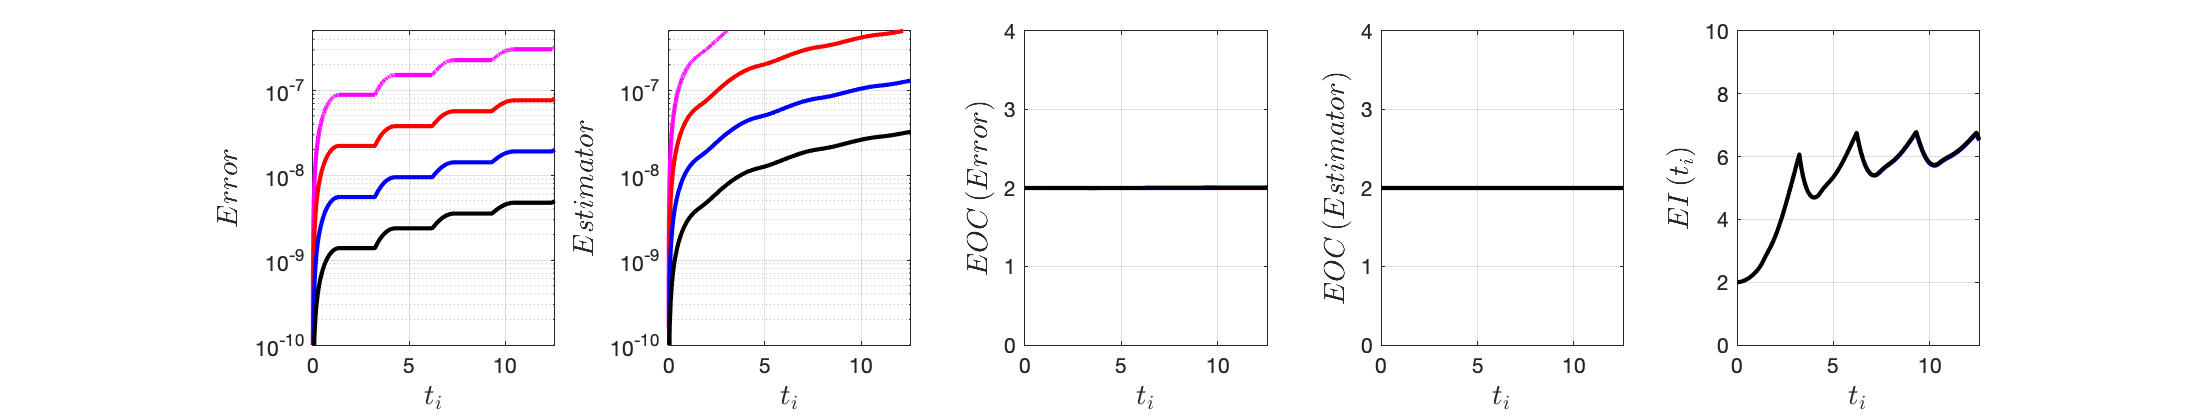
\includegraphics[scale=0.55]{fig_LeapFrogplots_1x5_sin_IC_harmonic_order_2_u0_v10_rec_george}	
	\caption{Reconstruction from Defn. \ref{defn_our_rec}. (from left to right) Error $e_R$ given by (\ref{eq_error_eR}), Estimator $\eta_1$ given by \ref{eq_bound_test}, Error $e_L$ given by  (\ref{eq_error_eL}). EOC error, EOC Estimator, Effectivity Index.}
	\label{fig_all_in_one_our_rec_george_u0_v10}
\end{figure}

\begin{figure}[H]
	\hspace{-3cm}
	%\centering
	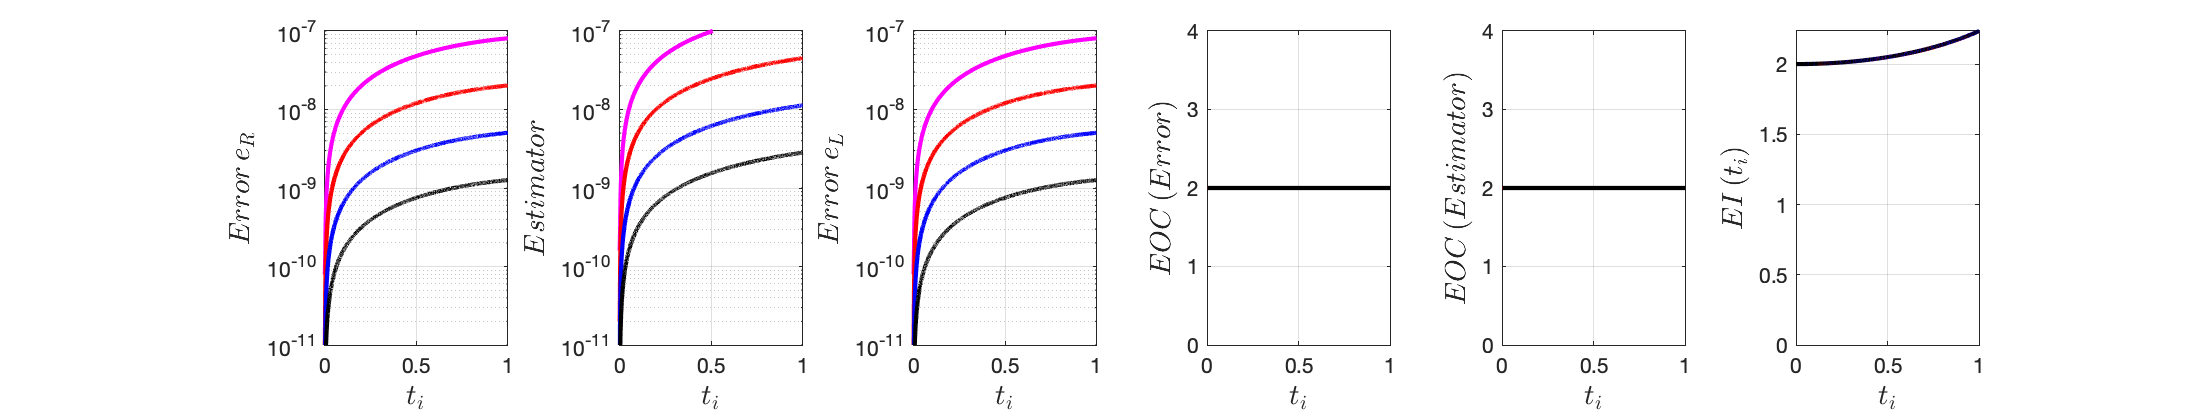
\includegraphics[scale=0.55]{fig_LeapFrogplots_1x5_sin_IC_harmonic_order_2_u0_v10_rec2}	
	\caption{Reconstruction from Defn. \ref{defn_our_rec2}. (from left to right) Error $e_R$ given by (\ref{eq_error_eR}), Estimator $\eta_1$ given by \ref{eq_bound_test}, Error $e_L$ given by  (\ref{eq_error_eL}). EOC error, EOC Estimator, Effectivity Index.}
	\label{fig_all_in_one_our_rec_2_u0_v10}
\end{figure}

\begin{figure}[H]
	\hspace{-3cm}
	%\centering
	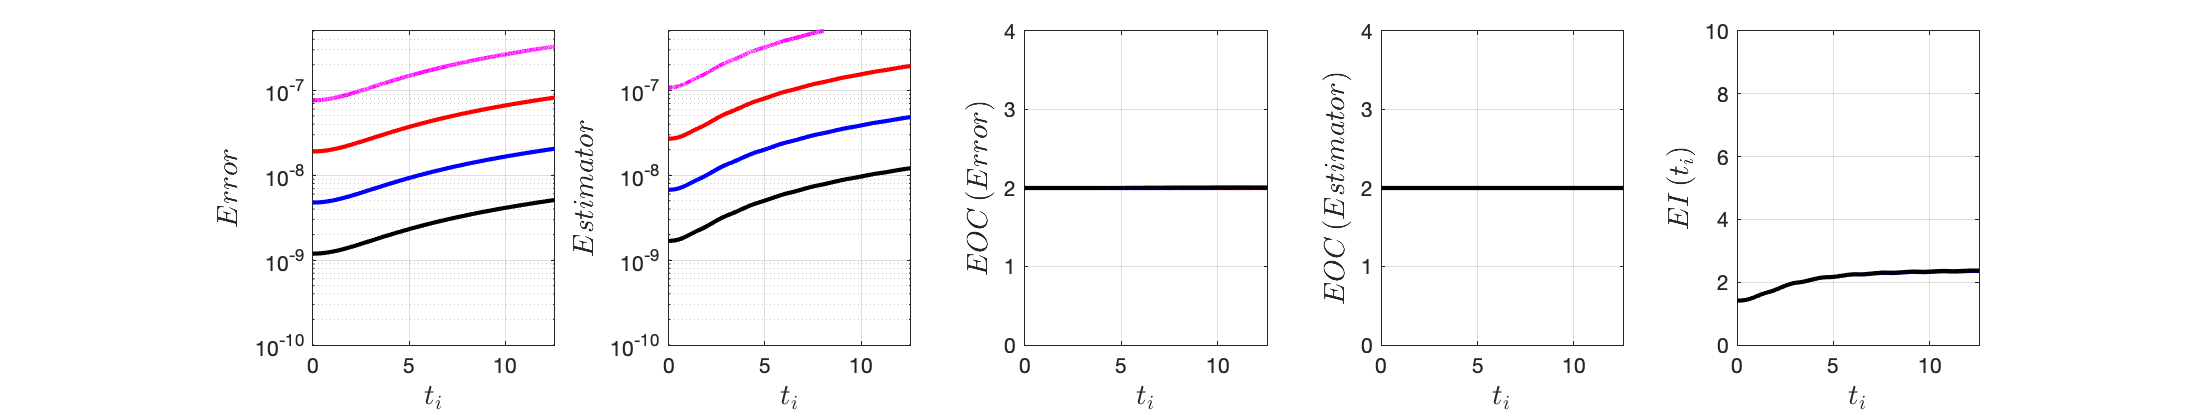
\includegraphics[scale=0.55]{fig_LeapFrogplots_1x5_sin_IC_harmonic_u0_v10_paperrec}	
	\caption{Paper rec. (from left to right) Error $e_R$ given by (\ref{eq_error_eR}), Estimator $\eta_1$ given by \ref{eq_bound_test}, Error $e_L$ given by  (\ref{eq_error_eL}). EOC error, EOC Estimator, Effectivity Index.}
	\label{fig_all_in_one_paperrec_u0_v10}
\end{figure}

\subsection{$u_0=0.1, v_0= 0.9$}

\begin{figure}[H]
	\hspace{-3cm}
	%\centering
	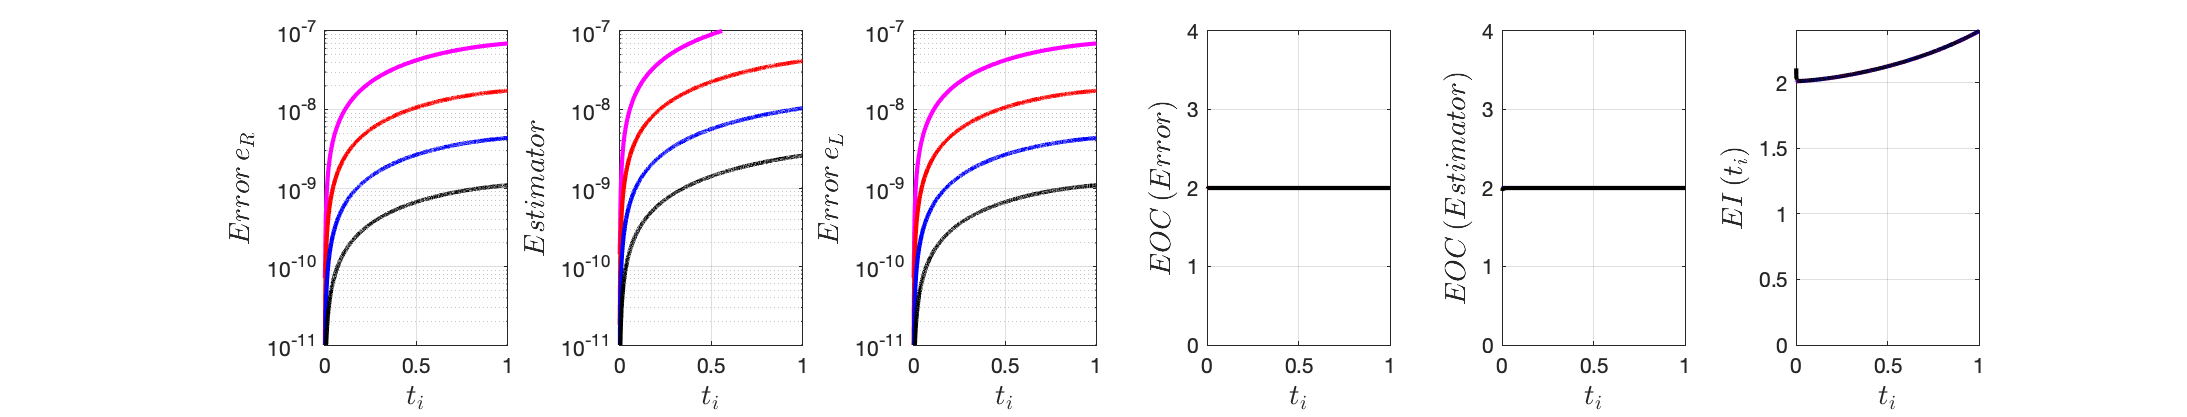
\includegraphics[scale=0.55]{fig_LeapFrogplots_1x5_sin_IC_harmonic_order_2_u1_v9_rec_george}	
	\caption{Reconstruction from Defn. \ref{defn_our_rec}. (from left to right) Error $e_R$ given by (\ref{eq_error_eR}), Estimator $\eta_1$ given by \ref{eq_bound_test}, Error $e_L$ given by  (\ref{eq_error_eL}). EOC error, EOC Estimator, Effectivity Index.}
	\label{fig_all_in_one_our_rec_george_u1_v9}
\end{figure}

\begin{figure}[H]
	\hspace{-3cm}
	%\centering
	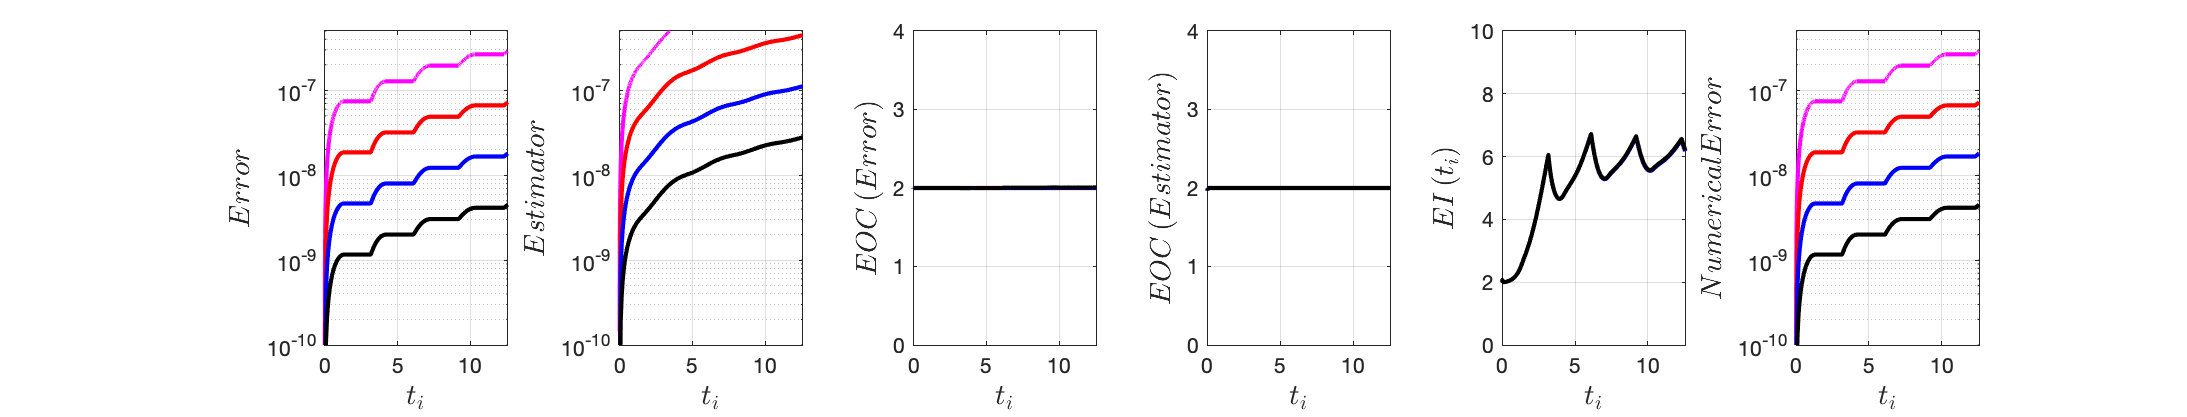
\includegraphics[scale=0.55]{fig_LeapFrogplots_1x5_sin_IC_harmonic_order_2_u1_v9_rec2}	
	\caption{Reconstruction from Defn. \ref{defn_our_rec2}. (from left to right) Error $e_R$ given by (\ref{eq_error_eR}), Estimator $\eta_1$ given by \ref{eq_bound_test}, Error $e_L$ given by  (\ref{eq_error_eL}). EOC error, EOC Estimator, Effectivity Index.}
	\label{fig_all_in_one_our_rec_2_u1_v9}
\end{figure}
\begin{figure}[H]
	\hspace{-3cm}
	%\centering
	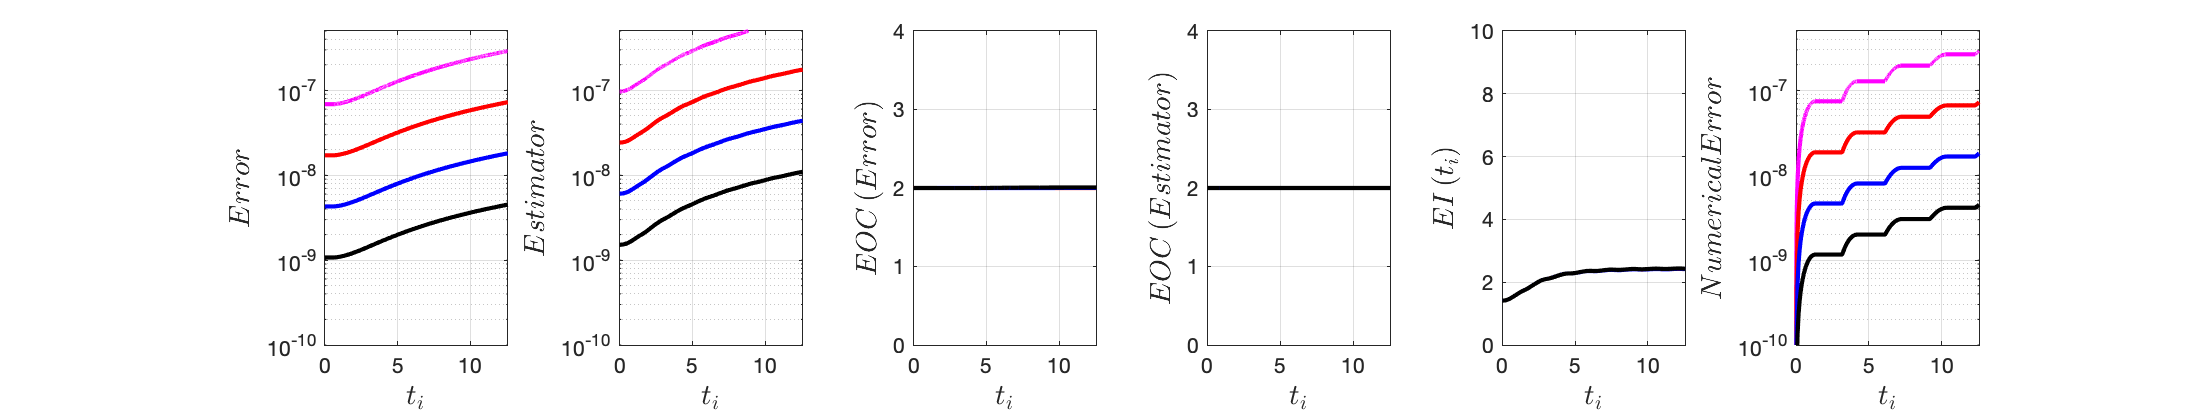
\includegraphics[scale=0.55]{fig_LeapFrogplots_1x5_sin_IC_harmonic_u1_v9_paperrec}	
	\caption{Paper rec. (from left to right) Error $e_R$ given by (\ref{eq_error_eR}), Estimator $\eta_1$ given by \ref{eq_bound_test}, Error $e_L$ given by  (\ref{eq_error_eL}). EOC error, EOC Estimator, Effectivity Index.}
	\label{fig_all_in_one_paperrec_u01_v09}
\end{figure}



\subsection{$u_0=0.2, v_0= 0.8$}
\begin{figure}[H]
	\hspace{-3cm}
	%\centering
	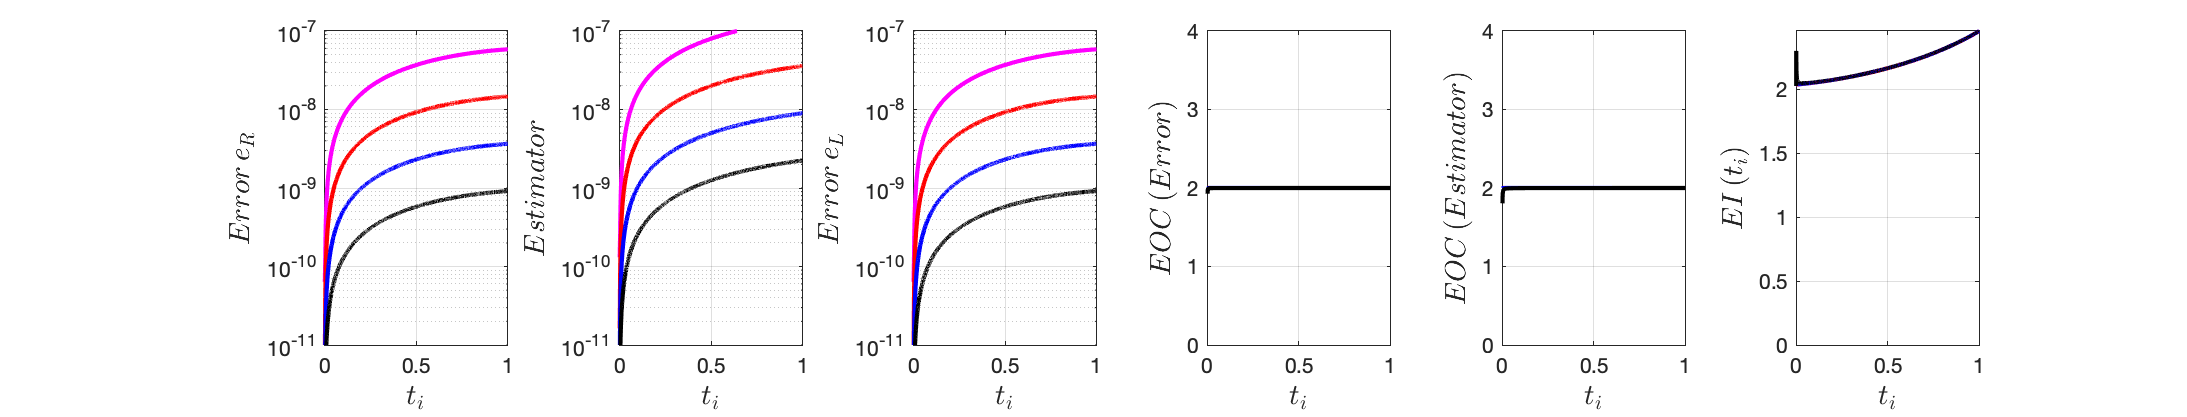
\includegraphics[scale=0.55]{fig_LeapFrogplots_1x5_sin_IC_harmonic_order_2_u2_v8_rec_george}	
	\caption{Reconstruction from Defn. \ref{defn_our_rec}. (from left to right) Error $e_R$ given by (\ref{eq_error_eR}), Estimator $\eta_1$ given by \ref{eq_bound_test}, Error $e_L$ given by  (\ref{eq_error_eL}). EOC error, EOC Estimator, Effectivity Index.}
	\label{fig_all_in_one_our_rec_george_u2_v8}
\end{figure}
\begin{figure}[H]
	\hspace{-3cm}
	%\centering
	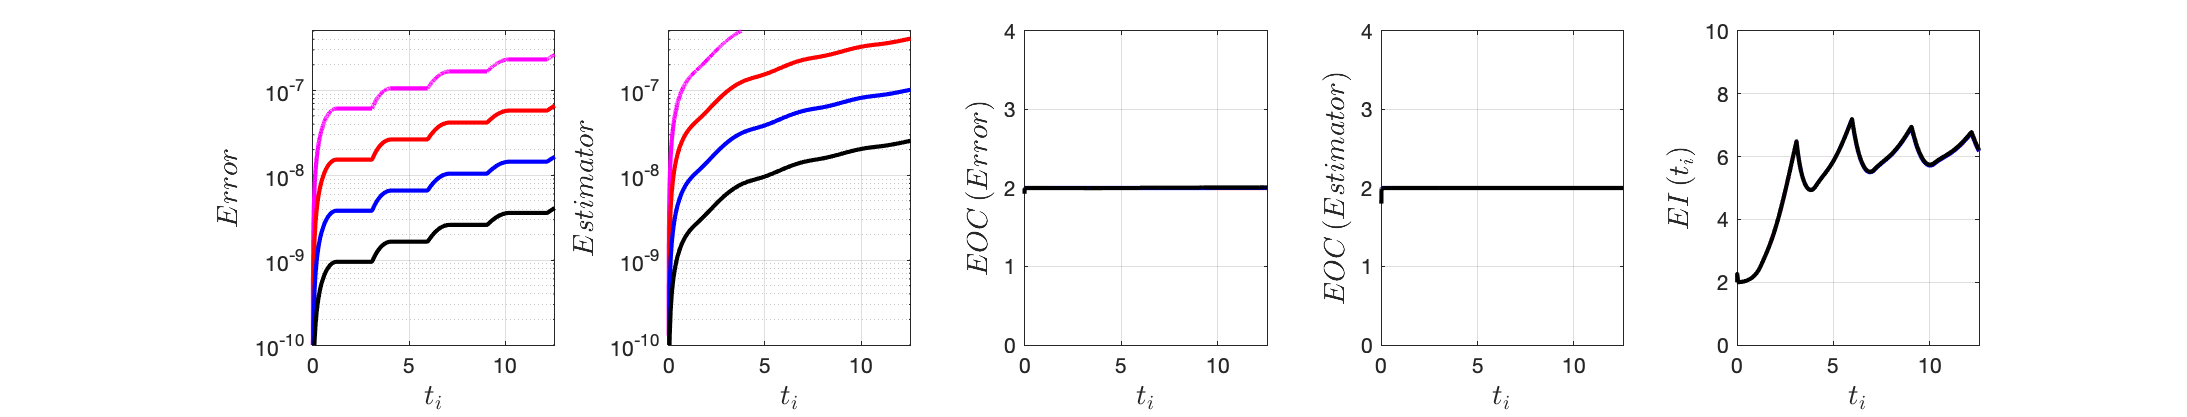
\includegraphics[scale=0.55]{fig_LeapFrogplots_1x5_sin_IC_harmonic_order_2_u2_v8_rec2}	
	\caption{Reconstruction from Defn. \ref{defn_our_rec2}. (from left to right) Error $e_R$ given by (\ref{eq_error_eR}), Estimator $\eta_1$ given by \ref{eq_bound_test}, Error $e_L$ given by  (\ref{eq_error_eL}). EOC error, EOC Estimator, Effectivity Index.}
	\label{fig_all_in_one_our_rec_2_u2_v8}
\end{figure}

\begin{figure}[H]
	\hspace{-3cm}
	%\centering
	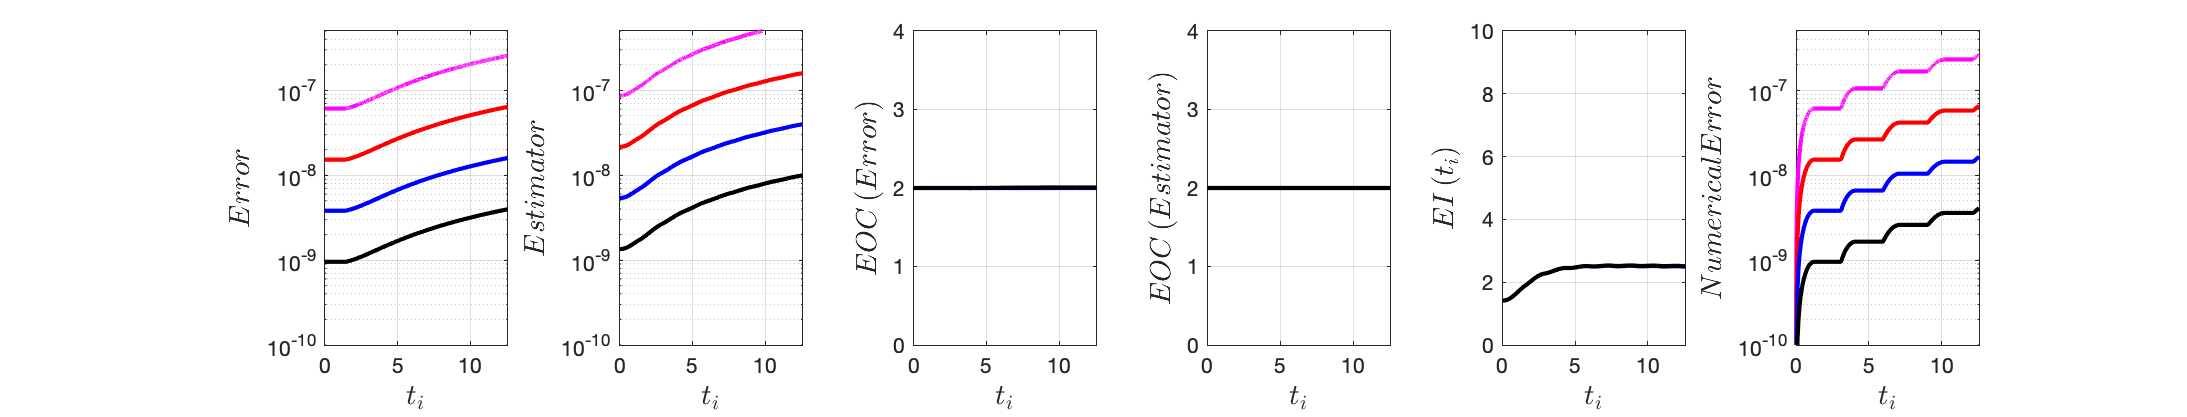
\includegraphics[scale=0.55]{fig_LeapFrogplots_1x5_sin_IC_harmonic_u2_v8_paperrec}	
	\caption{Paper rec. (from left to right) Error $e_R$ given by (\ref{eq_error_eR}), Estimator $\eta_1$ given by \ref{eq_bound_test}, Error $e_L$ given by  (\ref{eq_error_eL}). EOC error, EOC Estimator, Effectivity Index.}
	\label{fig_all_in_one_paperrec_u02_v08}
\end{figure}


\subsection{$u_0=0.3, v_0= 0.7$}
\begin{figure}[H]
	\hspace{-3cm}
	%\centering
	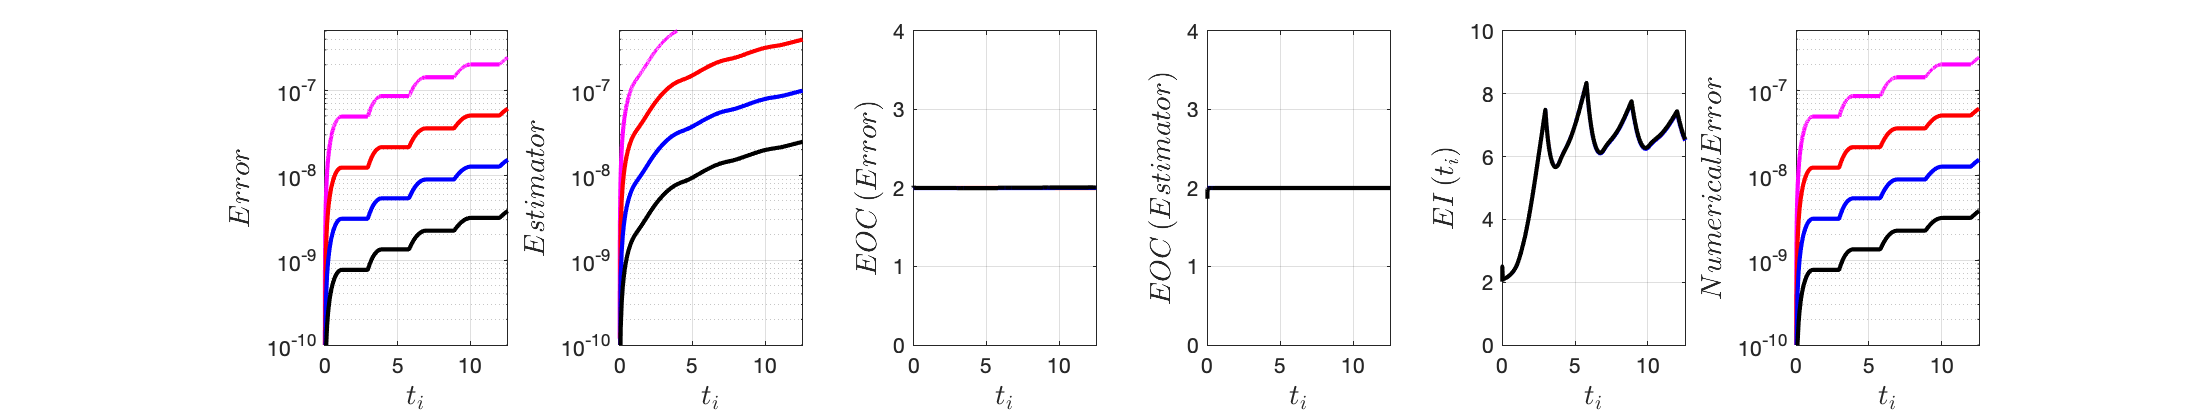
\includegraphics[scale=0.55]{fig_LeapFrogplots_1x5_sin_IC_harmonic_order_2_u3_v7_rec_george}	
	\caption{Reconstruction from Defn. \ref{defn_our_rec}. (from left to right) Error $e_R$ given by (\ref{eq_error_eR}), Estimator $\eta_1$ given by \ref{eq_bound_test}, Error $e_L$ given by  (\ref{eq_error_eL}). EOC error, EOC Estimator, Effectivity Index.}
	\label{fig_all_in_one_our_rec_george_u3_v7}
\end{figure}
\begin{figure}[H]
	\hspace{-3cm}
	%\centering
	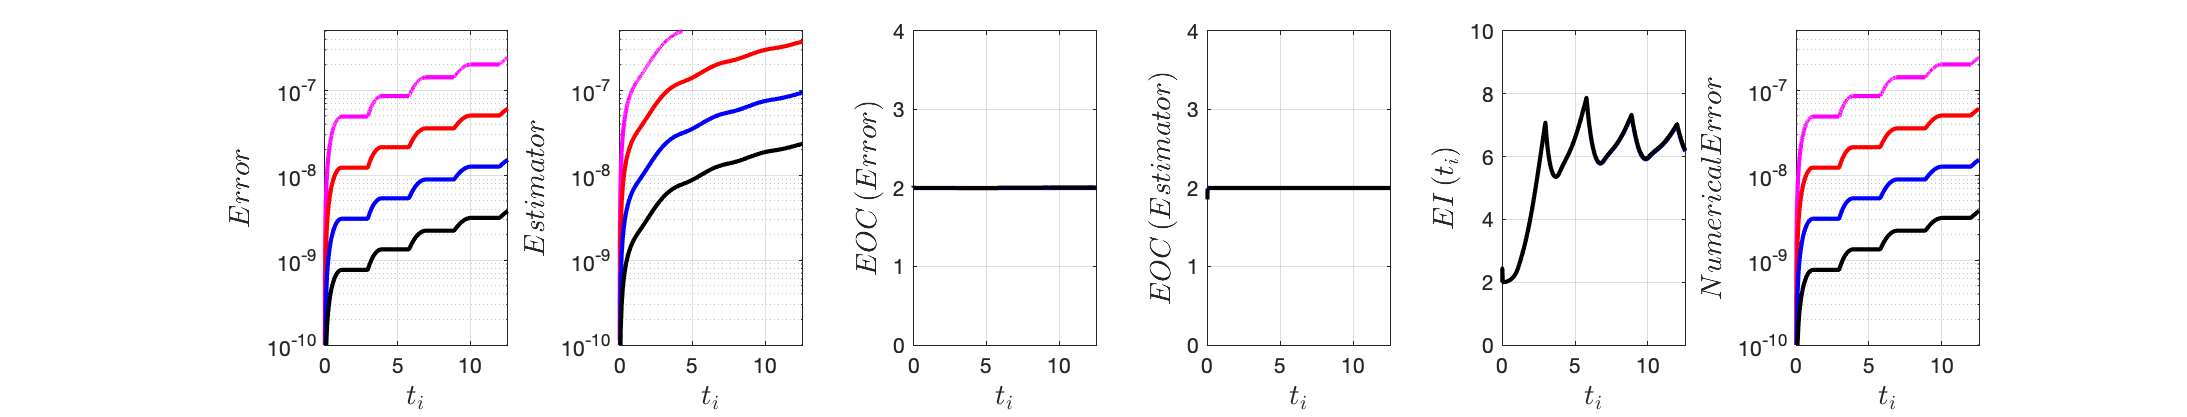
\includegraphics[scale=0.55]{fig_LeapFrogplots_1x5_sin_IC_harmonic_order_2_u3_v7_rec2}	
	\caption{Reconstruction from Defn. \ref{defn_our_rec2}. (from left to right) Error $e_R$ given by (\ref{eq_error_eR}), Estimator $\eta_1$ given by \ref{eq_bound_test}, Error $e_L$ given by  (\ref{eq_error_eL}). EOC error, EOC Estimator, Effectivity Index.}
	\label{fig_all_in_one_our_rec_2_u3_v7}
\end{figure}
\begin{figure}[H]
	\hspace{-3cm}
	%\centering
	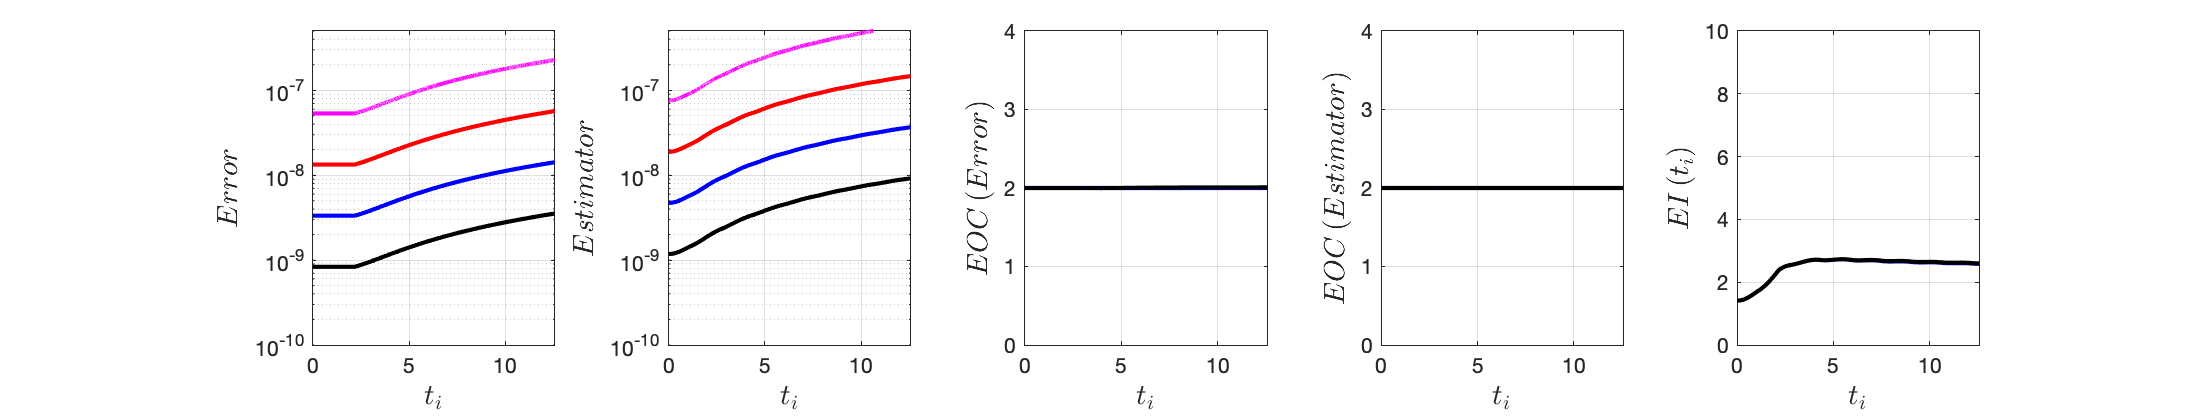
\includegraphics[scale=0.55]{fig_LeapFrogplots_1x5_sin_IC_harmonic_u3_v7_paperrec}	
	\caption{Paper rec. (from left to right) Error $e_R$ given by (\ref{eq_error_eR}), Estimator $\eta_1$ given by \ref{eq_bound_test}, Error $e_L$ given by  (\ref{eq_error_eL}). EOC error, EOC Estimator, Effectivity Index.}
	\label{fig_all_in_one_paperrec_u03_v07}
\end{figure}


\subsection{$u_0=0.4, v_0= 0.6$}
\begin{figure}[H]
	\hspace{-3cm}
	%\centering
	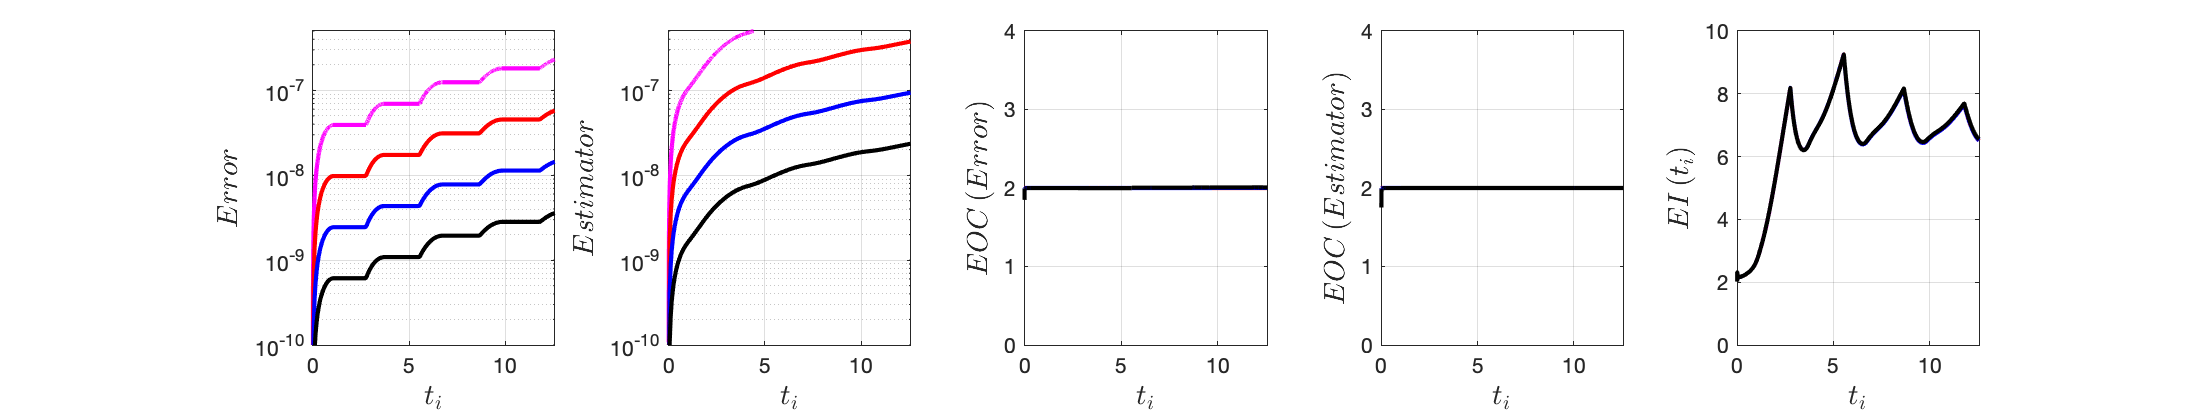
\includegraphics[scale=0.55]{fig_LeapFrogplots_1x5_sin_IC_harmonic_order_2_u4_v6_rec_george}	
	\caption{Reconstruction from Defn. \ref{defn_our_rec}. (from left to right) Error $e_R$ given by (\ref{eq_error_eR}), Estimator $\eta_1$ given by \ref{eq_bound_test}, Error $e_L$ given by  (\ref{eq_error_eL}). EOC error, EOC Estimator, Effectivity Index.}
	\label{fig_all_in_one_our_rec_george_u4_v6}
\end{figure}
\begin{figure}[H]
	\hspace{-3cm}
	%\centering
	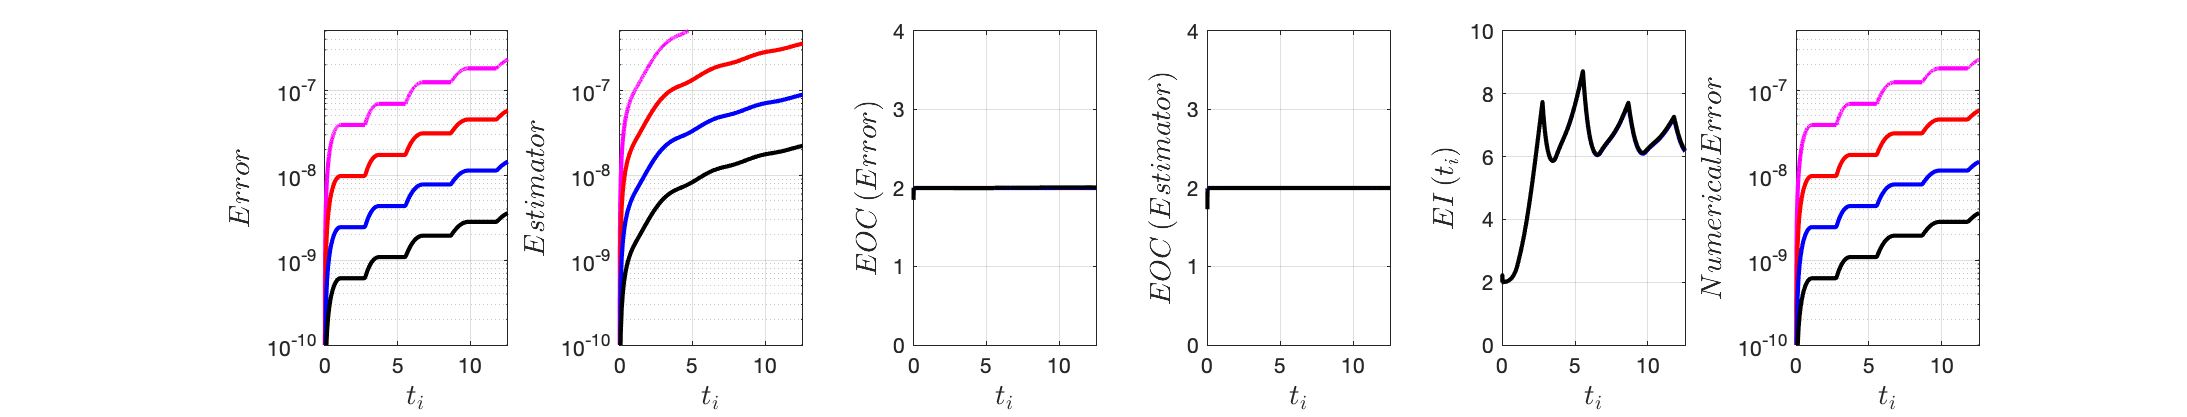
\includegraphics[scale=0.55]{fig_LeapFrogplots_1x5_sin_IC_harmonic_order_2_u4_v6_rec2}	
	\caption{Reconstruction from Defn. \ref{defn_our_rec2}. (from left to right) Error $e_R$ given by (\ref{eq_error_eR}), Estimator $\eta_1$ given by \ref{eq_bound_test}, Error $e_L$ given by  (\ref{eq_error_eL}). EOC error, EOC Estimator, Effectivity Index.}
	\label{fig_all_in_one_our_rec_2_u4_v6}
\end{figure}
\begin{figure}[H]
	\hspace{-3cm}
	%\centering
	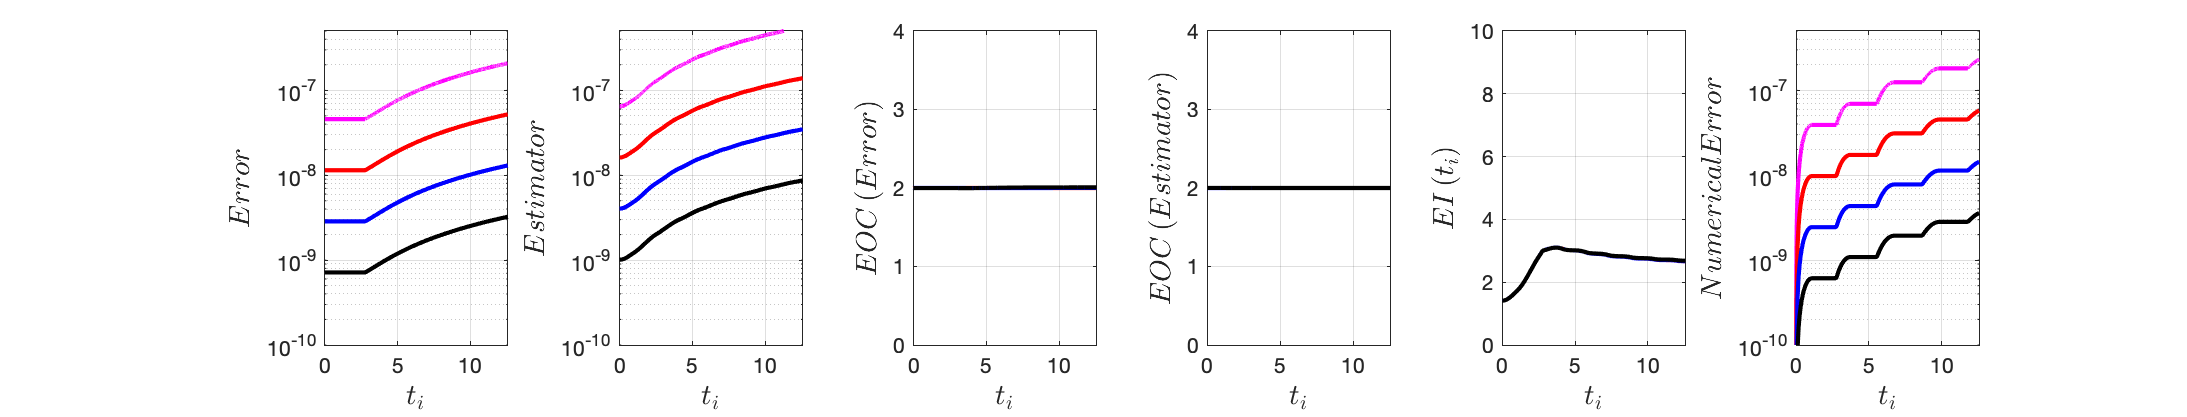
\includegraphics[scale=0.55]{fig_LeapFrogplots_1x5_sin_IC_harmonic_u4_v6_paperrec}	
	\caption{Paper rec. (from left to right) Error $e_R$ given by (\ref{eq_error_eR}), Estimator $\eta_1$ given by \ref{eq_bound_test}, Error $e_L$ given by  (\ref{eq_error_eL}). EOC error, EOC Estimator, Effectivity Index.}
	\label{fig_all_in_one_paperrec_u04_v06}
\end{figure}



\subsection{$u_0=0.5, v_0= 0.5$}
\begin{figure}[H]
	\hspace{-3cm}
	%\centering
	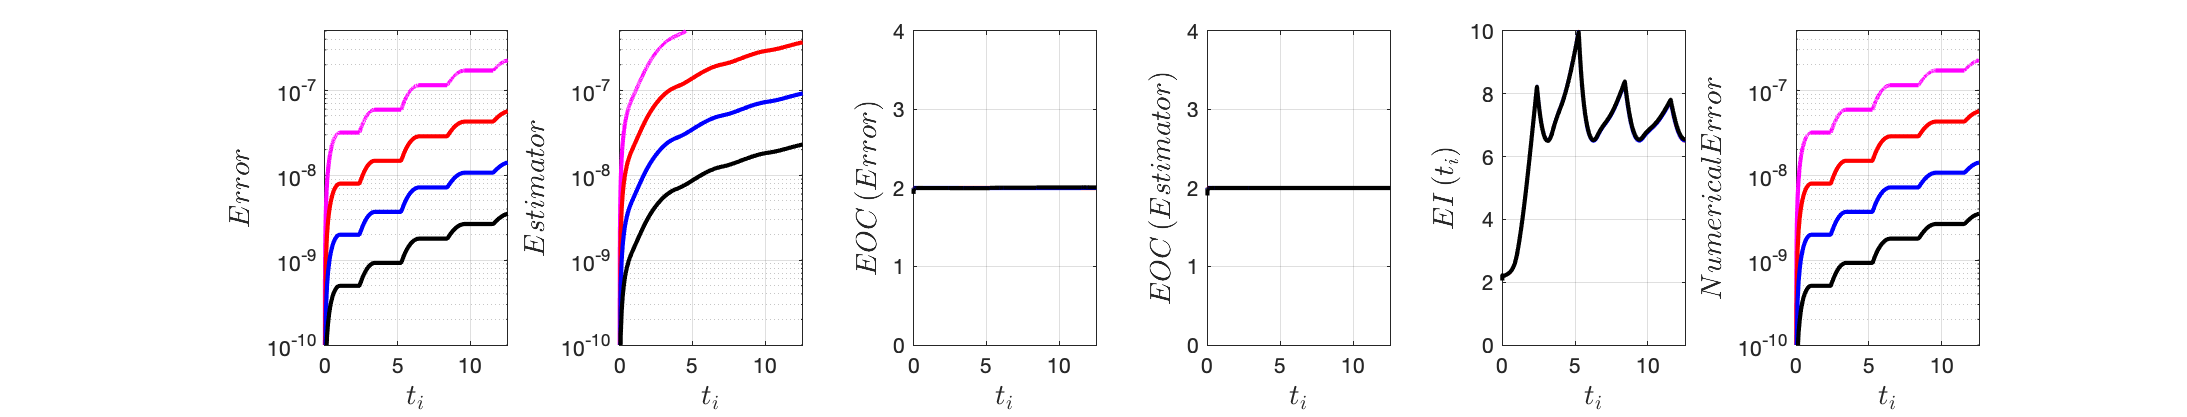
\includegraphics[scale=0.55]{fig_LeapFrogplots_1x5_sin_IC_harmonic_order_2_u5_v5_rec_george}	
	\caption{Reconstruction from Defn. \ref{defn_our_rec}. (from left to right) Error $e_R$ given by (\ref{eq_error_eR}), Estimator $\eta_1$ given by \ref{eq_bound_test}, Error $e_L$ given by  (\ref{eq_error_eL}). EOC error, EOC Estimator, Effectivity Index.}
	\label{fig_all_in_one_our_rec_george_u5_v5}
\end{figure}
\begin{figure}[H]
	\hspace{-3cm}
	%\centering
	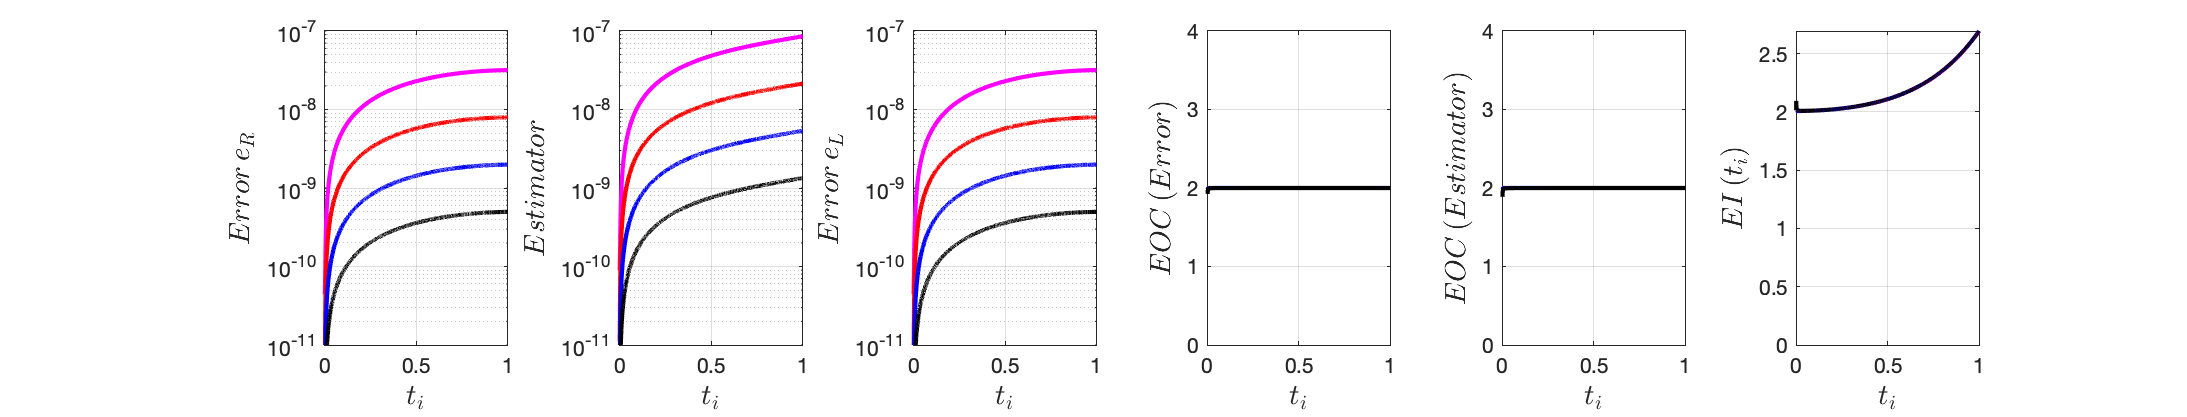
\includegraphics[scale=0.55]{fig_LeapFrogplots_1x5_sin_IC_harmonic_order_2_u5_v5_rec2}	
	\caption{Reconstruction from Defn. \ref{defn_our_rec2}. (from left to right) Error $e_R$ given by (\ref{eq_error_eR}), Estimator $\eta_1$ given by \ref{eq_bound_test}, Error $e_L$ given by  (\ref{eq_error_eL}). EOC error, EOC Estimator, Effectivity Index.}
	\label{fig_all_in_one_our_rec_2_u5_v5}
\end{figure}
\begin{figure}[H]
	\hspace{-3cm}
	%\centering
	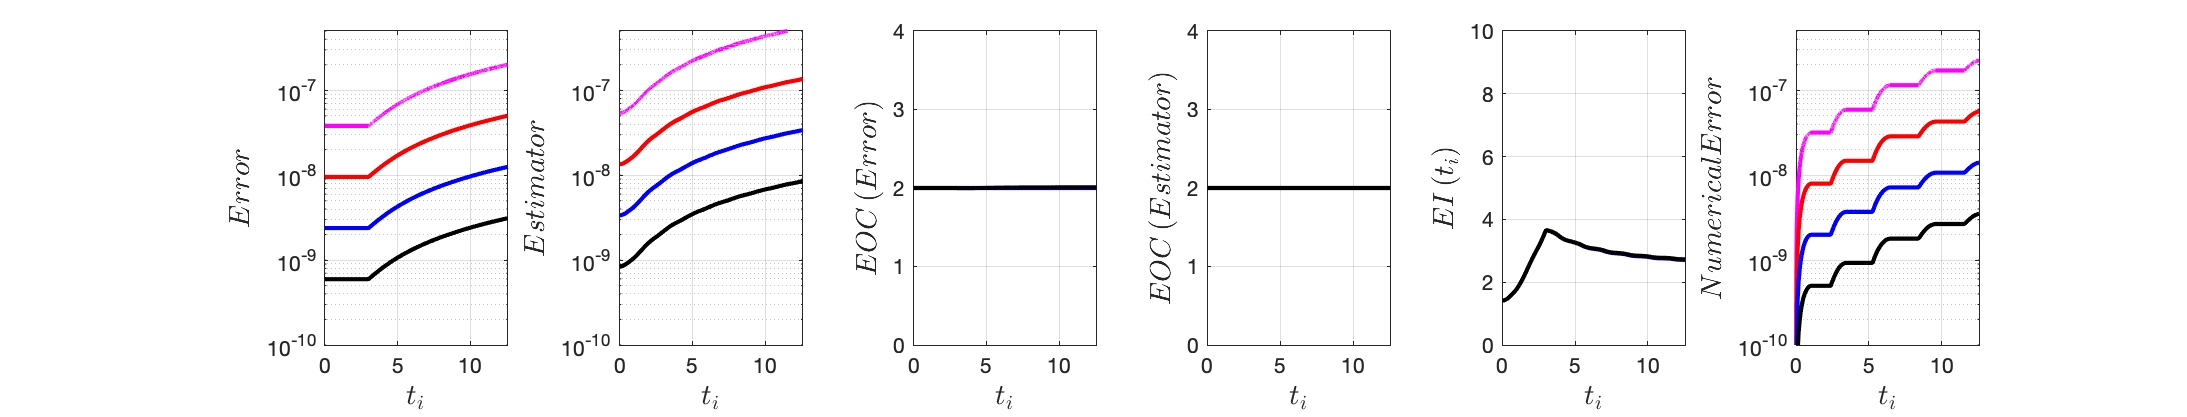
\includegraphics[scale=0.55]{fig_LeapFrogplots_1x5_sin_IC_harmonic_u5_v5_paperrec}	
	\caption{Paper rec. (from left to right) Error $e_R$ given by (\ref{eq_error_eR}), Estimator $\eta_1$ given by \ref{eq_bound_test}, Error $e_L$ given by  (\ref{eq_error_eL}). EOC error, EOC Estimator, Effectivity Index.}
	\label{fig_all_in_one_paperrec_u05_v05}
\end{figure}

\subsection{$u_0=0.6, v_0= 0.4$}
\begin{figure}[H]
	\hspace{-3cm}
	%\centering
	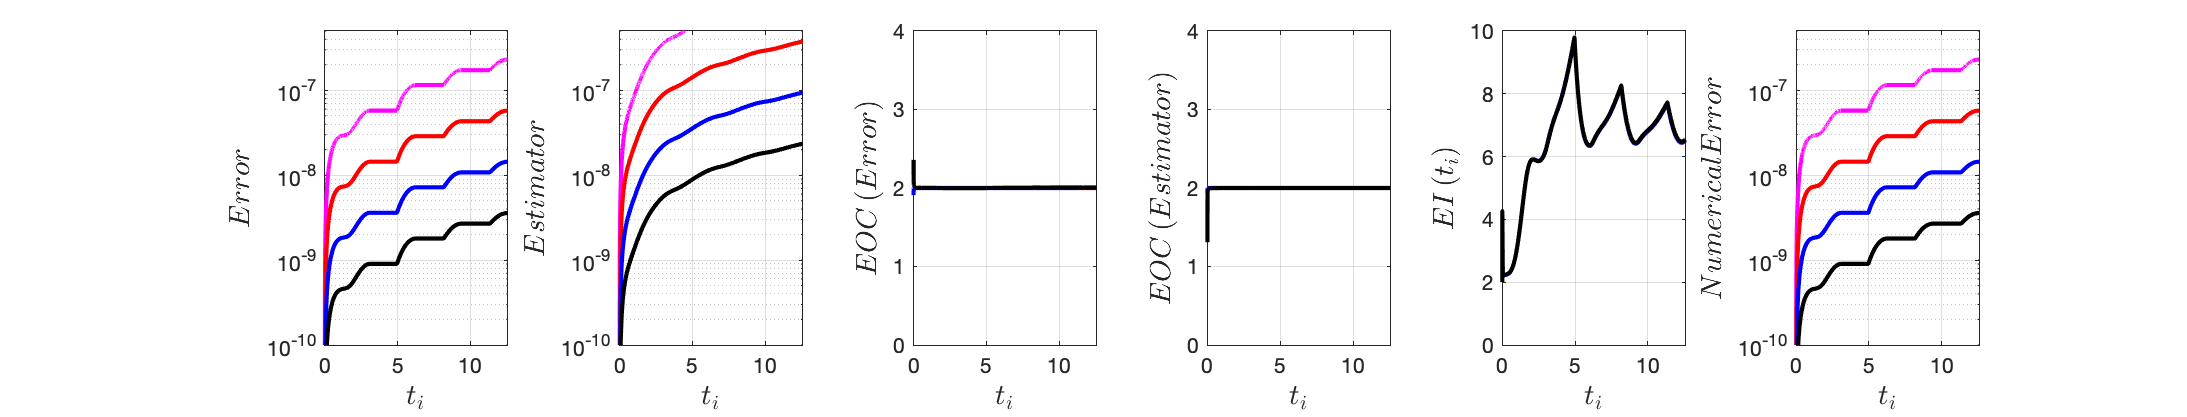
\includegraphics[scale=0.55]{fig_LeapFrogplots_1x5_sin_IC_harmonic_order_2_u6_v4_rec_george}	
	\caption{Reconstruction from Defn. \ref{defn_our_rec}. (from left to right) Error $e_R$ given by (\ref{eq_error_eR}), Estimator $\eta_1$ given by \ref{eq_bound_test}, Error $e_L$ given by  (\ref{eq_error_eL}). EOC error, EOC Estimator, Effectivity Index.}
	\label{fig_all_in_one_our_rec_george_u6_v4}
\end{figure}
\begin{figure}[H]
	\hspace{-3cm}
	%\centering
	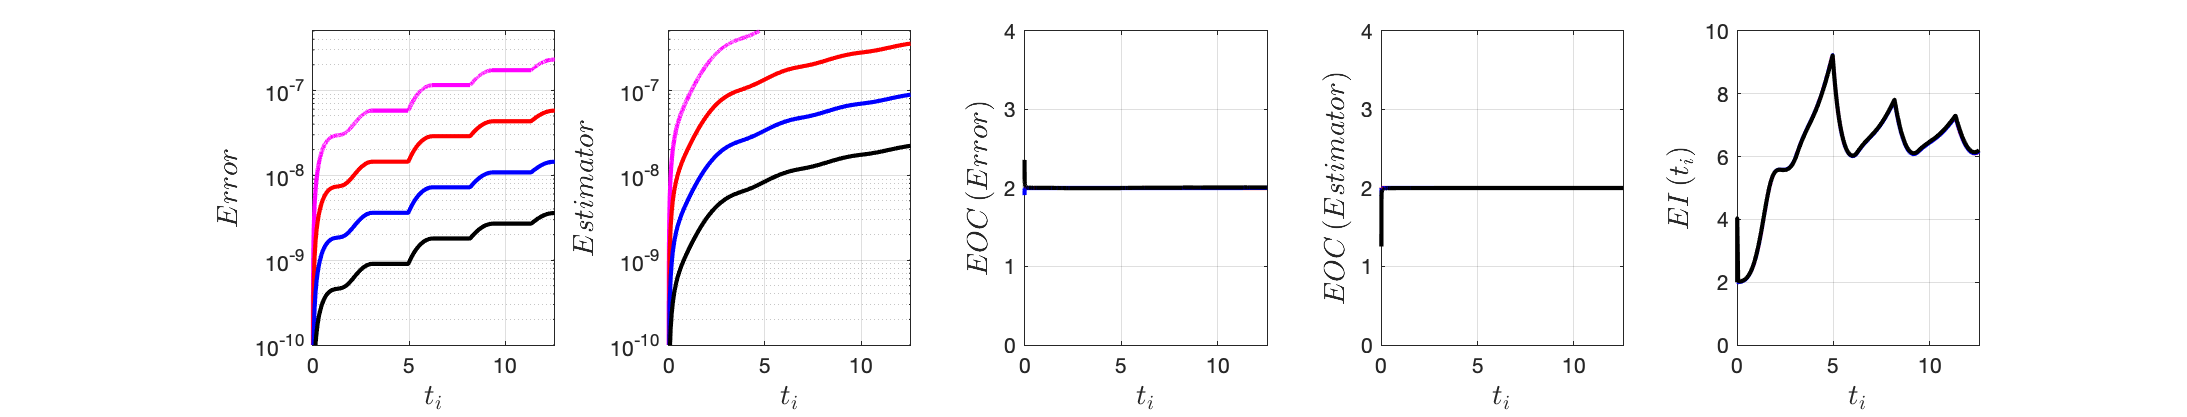
\includegraphics[scale=0.55]{fig_LeapFrogplots_1x5_sin_IC_harmonic_order_2_u6_v4_rec2}	
	\caption{Reconstruction from Defn. \ref{defn_our_rec2}. (from left to right) Error $e_R$ given by (\ref{eq_error_eR}), Estimator $\eta_1$ given by \ref{eq_bound_test}, Error $e_L$ given by  (\ref{eq_error_eL}). EOC error, EOC Estimator, Effectivity Index.}
	\label{fig_all_in_one_our_rec_2_u6_v4}
\end{figure}
\begin{figure}[H]
	\hspace{-3cm}
	%\centering
	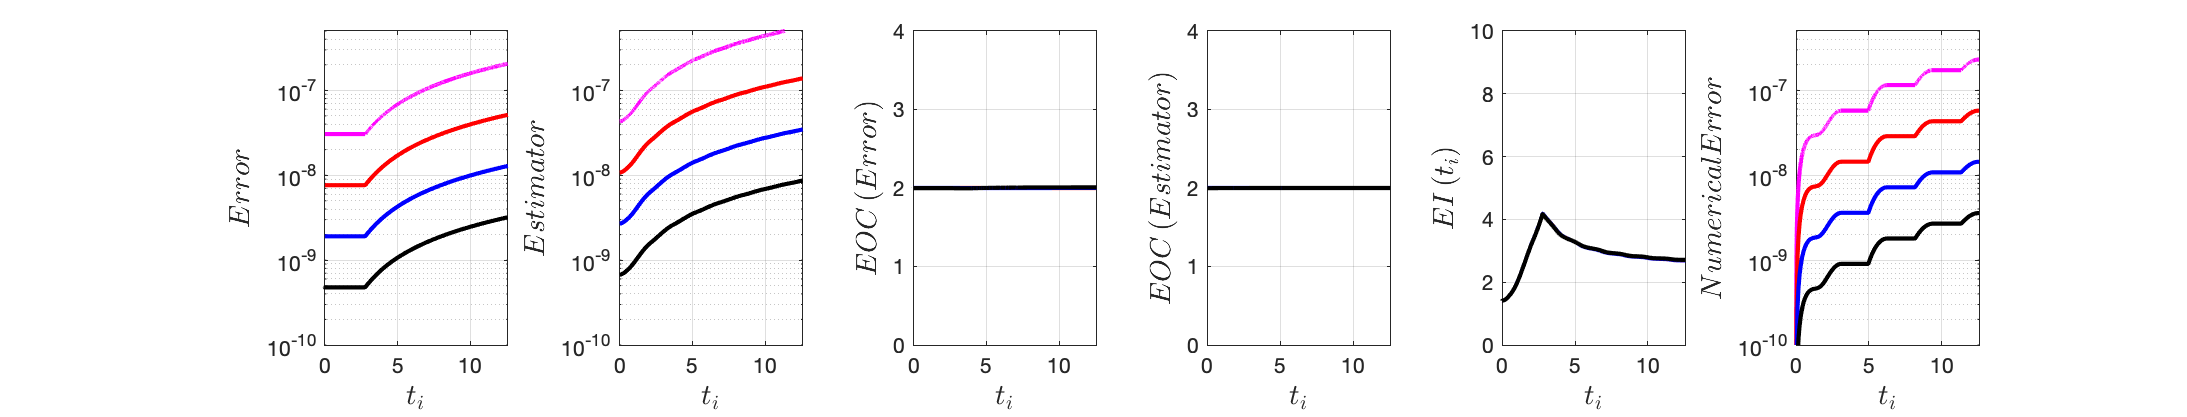
\includegraphics[scale=0.55]{fig_LeapFrogplots_1x5_sin_IC_harmonic_u6_v4_paperrec}	
	\caption{Paper rec. (from left to right) Error $e_R$ given by (\ref{eq_error_eR}), Estimator $\eta_1$ given by \ref{eq_bound_test}, Error $e_L$ given by  (\ref{eq_error_eL}). EOC error, EOC Estimator, Effectivity Index.}
	\label{fig_all_in_one_paperrec_u06_v04}
\end{figure}

\subsection{$u_0=0.7, v_0= 0.3$}
\begin{figure}[H]
	\hspace{-3cm}
	%\centering
	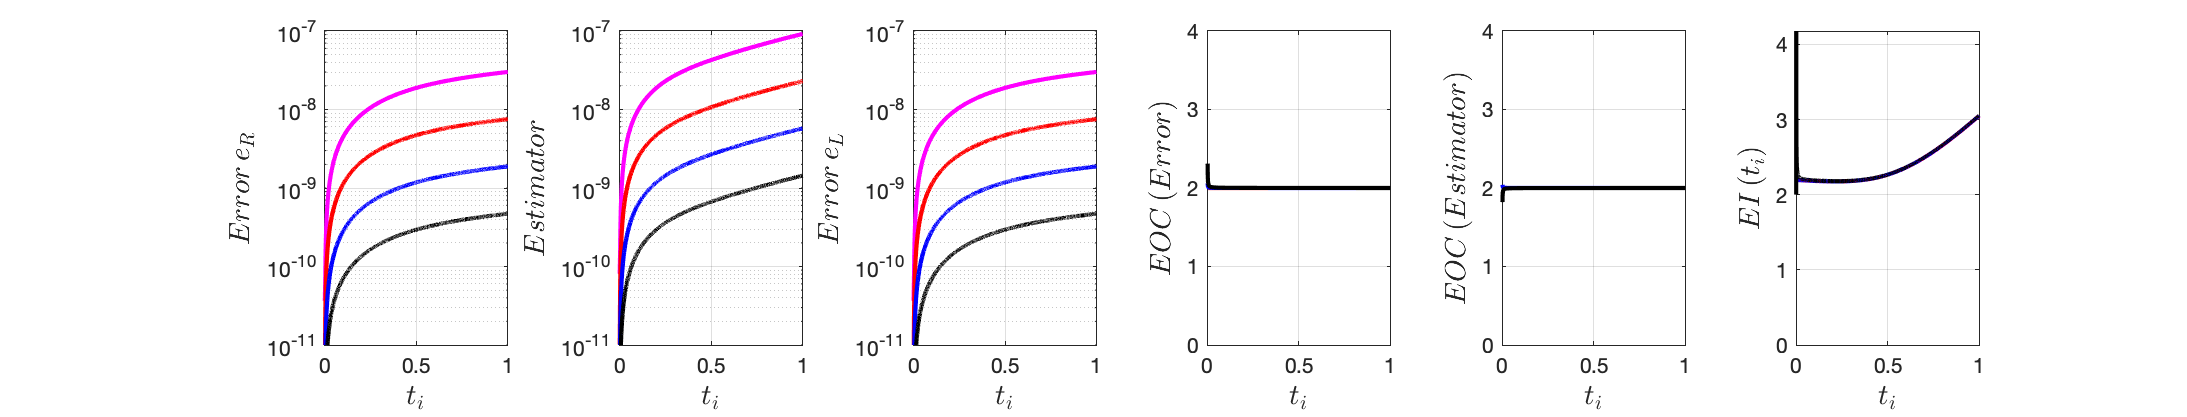
\includegraphics[scale=0.55]{fig_LeapFrogplots_1x5_sin_IC_harmonic_order_2_u7_v3_rec_george}	
	\caption{Reconstruction from Defn. \ref{defn_our_rec}. (from left to right) Error $e_R$ given by (\ref{eq_error_eR}), Estimator $\eta_1$ given by \ref{eq_bound_test}, Error $e_L$ given by  (\ref{eq_error_eL}). EOC error, EOC Estimator, Effectivity Index.}
	\label{fig_all_in_one_our_rec_george_u7_v3}
\end{figure}
\begin{figure}[H]
	\hspace{-3cm}
	%\centering
	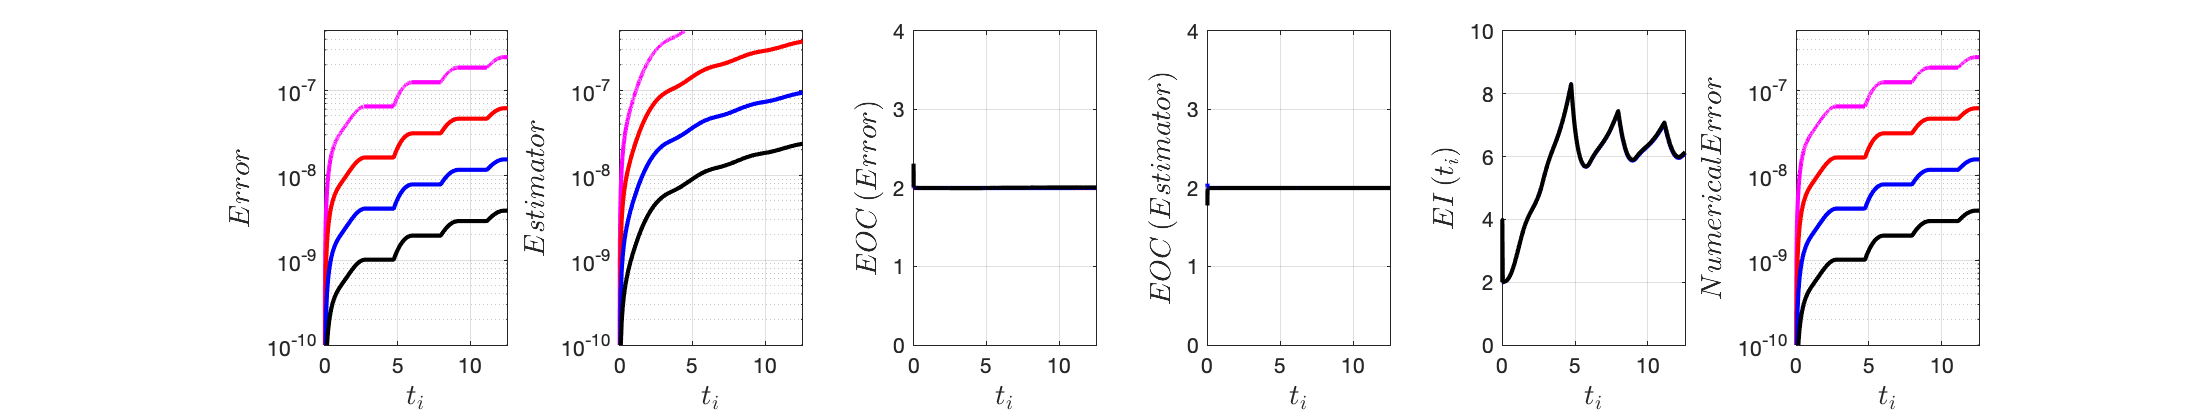
\includegraphics[scale=0.55]{fig_LeapFrogplots_1x5_sin_IC_harmonic_order_2_u7_v3_rec2}	
	\caption{Reconstruction from Defn. \ref{defn_our_rec2}. (from left to right) Error $e_R$ given by (\ref{eq_error_eR}), Estimator $\eta_1$ given by \ref{eq_bound_test}, Error $e_L$ given by  (\ref{eq_error_eL}). EOC error, EOC Estimator, Effectivity Index.}
	\label{fig_all_in_one_our_rec_2_u7_v3}
\end{figure}
\begin{figure}[H]
	\hspace{-3cm}
	%\centering
	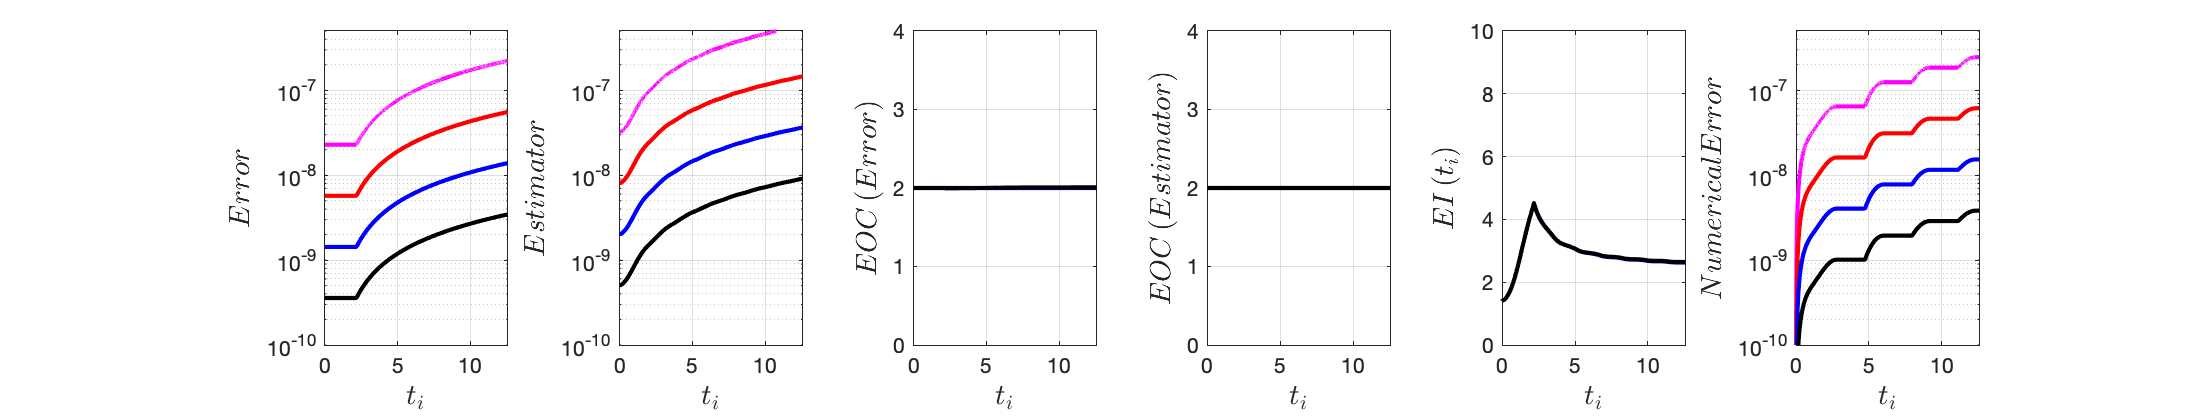
\includegraphics[scale=0.55]{fig_LeapFrogplots_1x5_sin_IC_harmonic_u7_v3_paperrec}	
	\caption{Paper rec. (from left to right) Error $e_R$ given by (\ref{eq_error_eR}), Estimator $\eta_1$ given by \ref{eq_bound_test}, Error $e_L$ given by  (\ref{eq_error_eL}). EOC error, EOC Estimator, Effectivity Index.}
	\label{fig_all_in_one_paperrec_u07_v03}
\end{figure}

\subsection{$u_0=0.8, v_0= 0.2$}
\begin{figure}[H]
	\hspace{-3cm}
	%\centering
	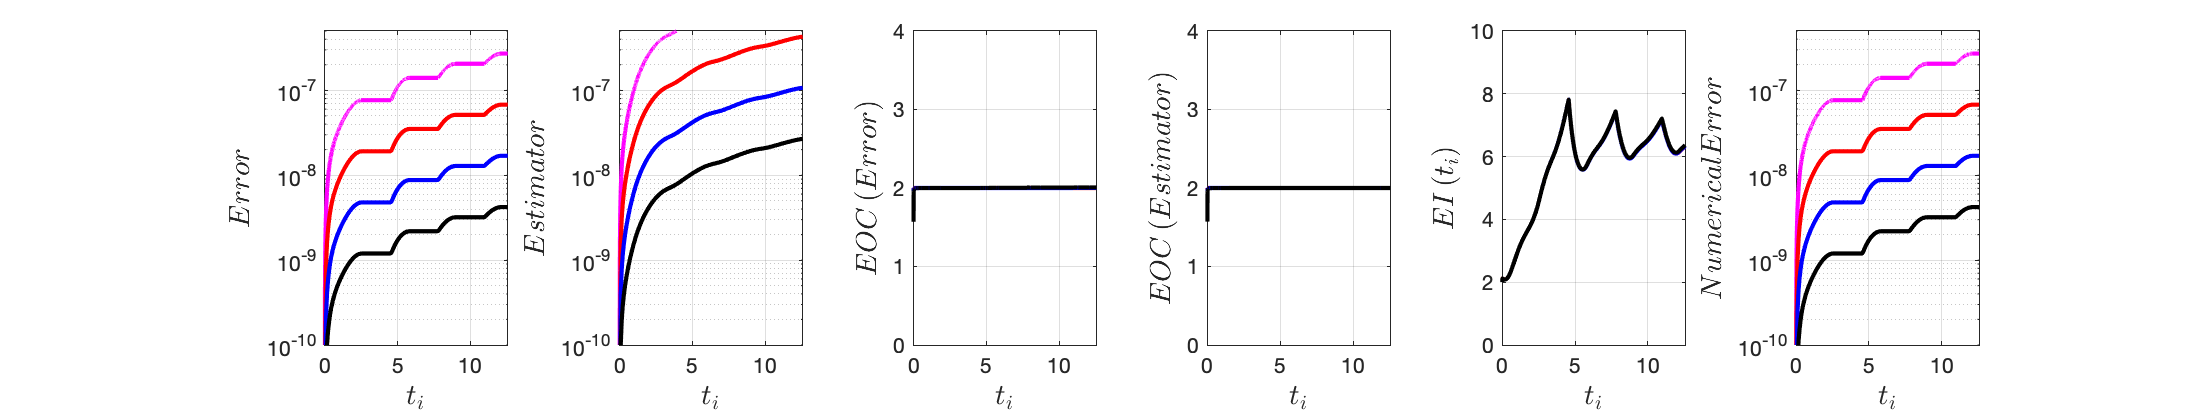
\includegraphics[scale=0.55]{fig_LeapFrogplots_1x5_sin_IC_harmonic_order_2_u8_v2_rec_george}	
	\caption{Reconstruction from Defn. \ref{defn_our_rec}. (from left to right) Error $e_R$ given by (\ref{eq_error_eR}), Estimator $\eta_1$ given by \ref{eq_bound_test}, Error $e_L$ given by  (\ref{eq_error_eL}). EOC error, EOC Estimator, Effectivity Index.}
	\label{fig_all_in_one_our_rec_george_u8_v2}
\end{figure}
\begin{figure}[H]
	\hspace{-3cm}
	%\centering
	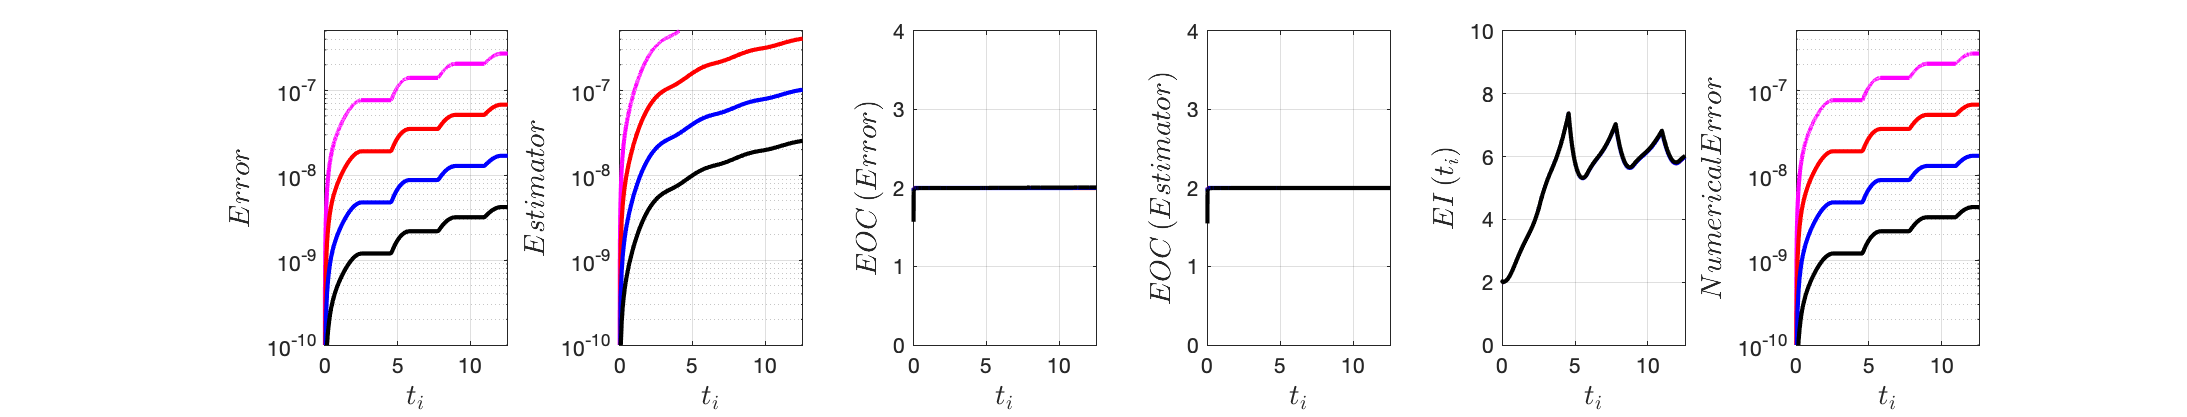
\includegraphics[scale=0.55]{fig_LeapFrogplots_1x5_sin_IC_harmonic_order_2_u8_v2_rec2}	
	\caption{Reconstruction from Defn. \ref{defn_our_rec2}. (from left to right) Error $e_R$ given by (\ref{eq_error_eR}), Estimator $\eta_1$ given by \ref{eq_bound_test}, Error $e_L$ given by  (\ref{eq_error_eL}). EOC error, EOC Estimator, Effectivity Index.}
	\label{fig_all_in_one_our_rec_2_u8_v2}
\end{figure}
\begin{figure}[H]
	\hspace{-3cm}
	%\centering
	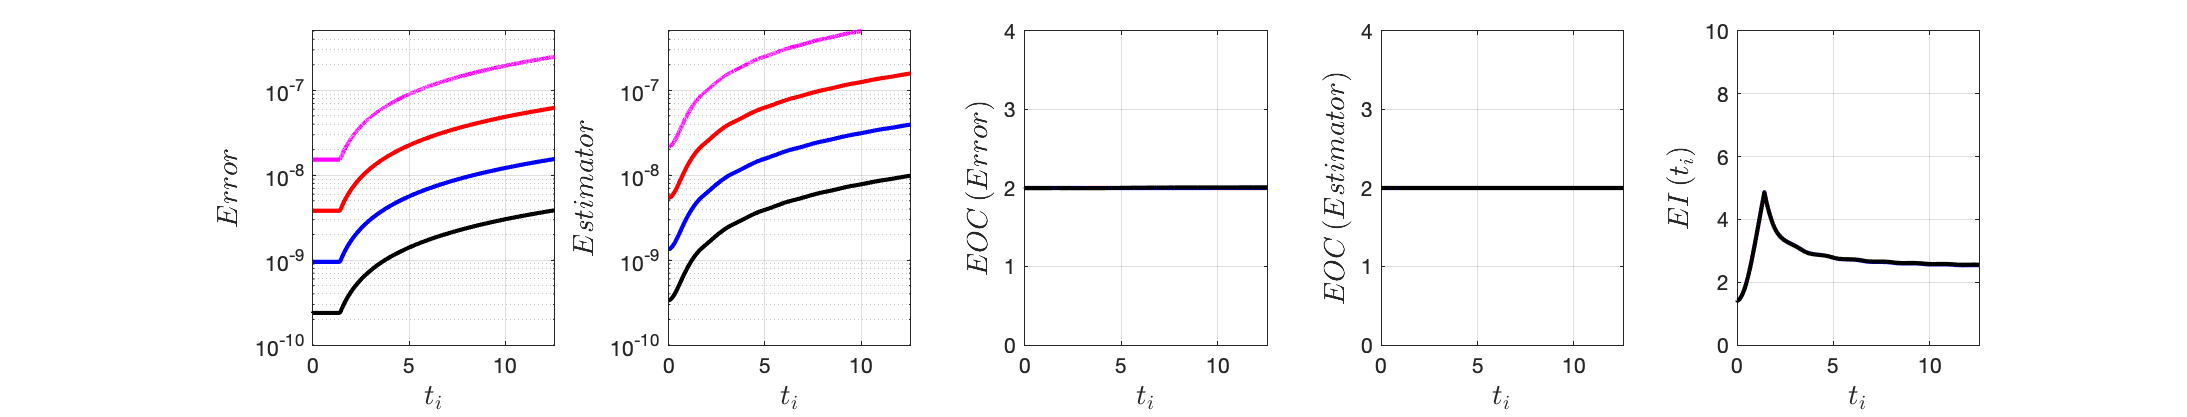
\includegraphics[scale=0.55]{fig_LeapFrogplots_1x5_sin_IC_harmonic_u8_v2_paperrec}	
	\caption{Paper rec. (from left to right) Error $e_R$ given by (\ref{eq_error_eR}), Estimator $\eta_1$ given by \ref{eq_bound_test}, Error $e_L$ given by  (\ref{eq_error_eL}). EOC error, EOC Estimator, Effectivity Index.}
	\label{fig_all_in_one_paperrec_u08_v02}
\end{figure}


\subsection{$u_0=0.9, v_0= 0.1$}
\begin{figure}[H]
	\hspace{-3cm}
	%\centering
	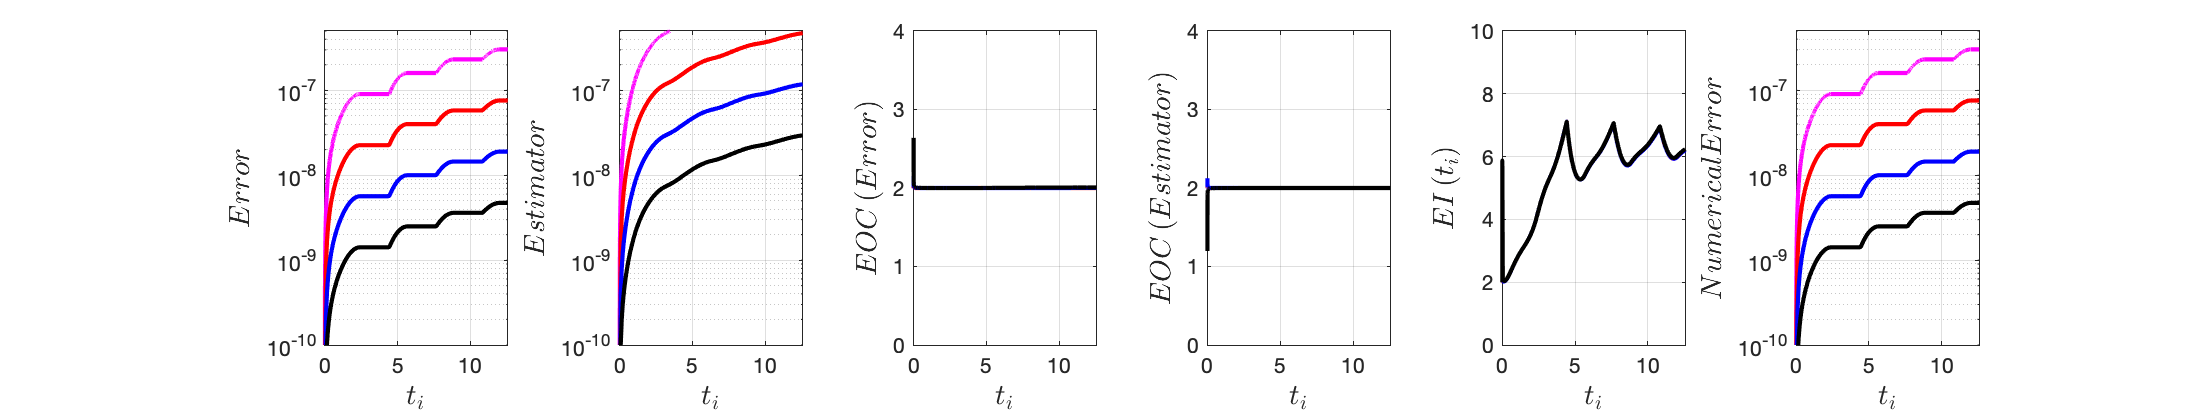
\includegraphics[scale=0.55]{fig_LeapFrogplots_1x5_sin_IC_harmonic_order_2_u9_v1_rec_george}	
	\caption{Reconstruction from Defn. \ref{defn_our_rec}. (from left to right) Error $e_R$ given by (\ref{eq_error_eR}), Estimator $\eta_1$ given by \ref{eq_bound_test}, Error $e_L$ given by  (\ref{eq_error_eL}). EOC error, EOC Estimator, Effectivity Index.}
	\label{fig_all_in_one_our_rec_george_u9_v1}
\end{figure}
\begin{figure}[H]
	\hspace{-3cm}
	%\centering
	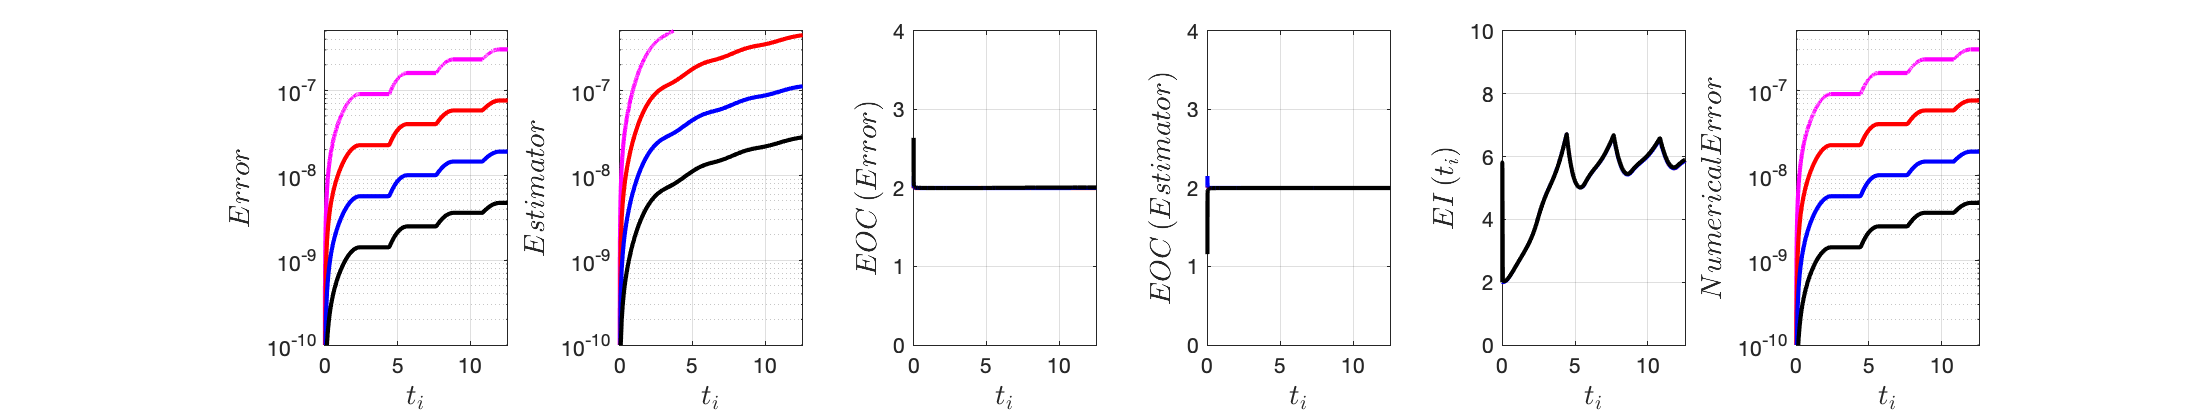
\includegraphics[scale=0.55]{fig_LeapFrogplots_1x5_sin_IC_harmonic_order_2_u9_v1_rec2}	
	\caption{Reconstruction from Defn. \ref{defn_our_rec2}. (from left to right) Error $e_R$ given by (\ref{eq_error_eR}), Estimator $\eta_1$ given by \ref{eq_bound_test}, Error $e_L$ given by  (\ref{eq_error_eL}). EOC error, EOC Estimator, Effectivity Index.}
	\label{fig_all_in_one_our_rec_2_u9_v1}
\end{figure}
\begin{figure}[H]
	\hspace{-3cm}
	%\centering
	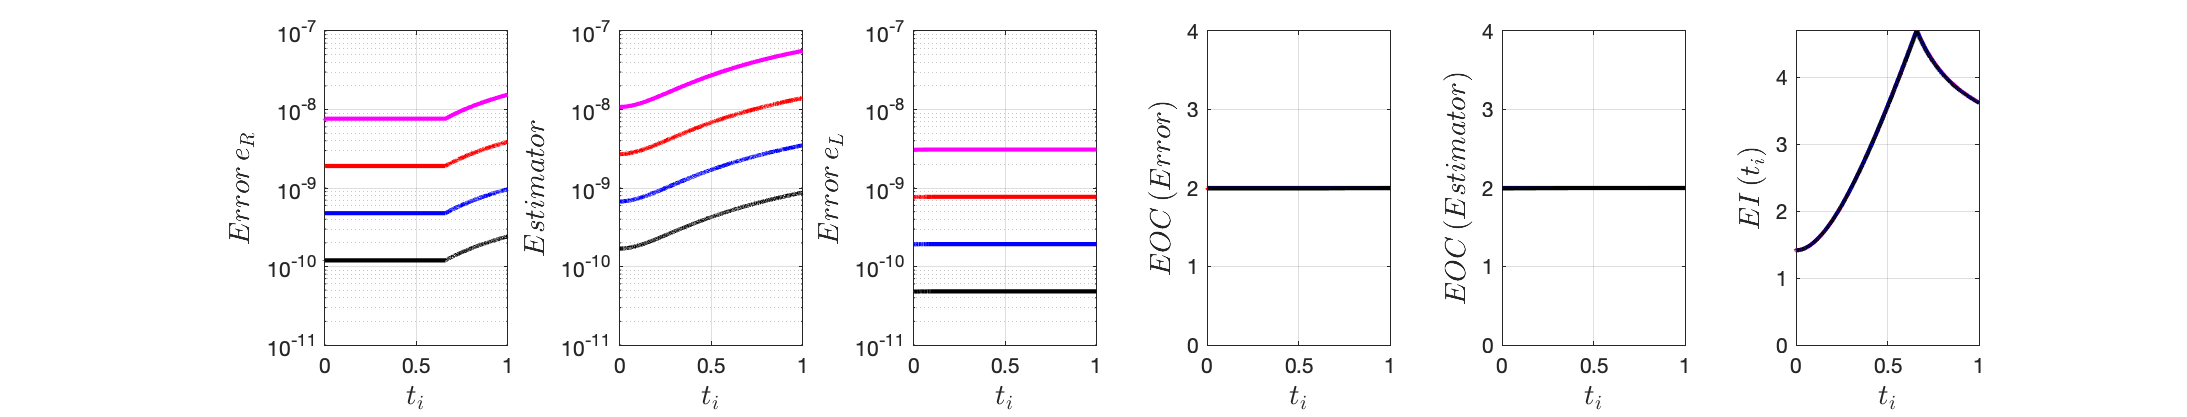
\includegraphics[scale=0.55]{fig_LeapFrogplots_1x5_sin_IC_harmonic_u9_v1_paperrec}	
	\caption{Paper rec. (from left to right) Error $e_R$ given by (\ref{eq_error_eR}), Estimator $\eta_1$ given by \ref{eq_bound_test}, Error $e_L$ given by  (\ref{eq_error_eL}). EOC error, EOC Estimator, Effectivity Index.}
	\label{fig_all_in_one_paperrec_u09_v01}
\end{figure}


\subsection{$u_0=1.0, v_0= 0$}
\begin{figure}[H]
	\hspace{-3cm}
	%\centering
	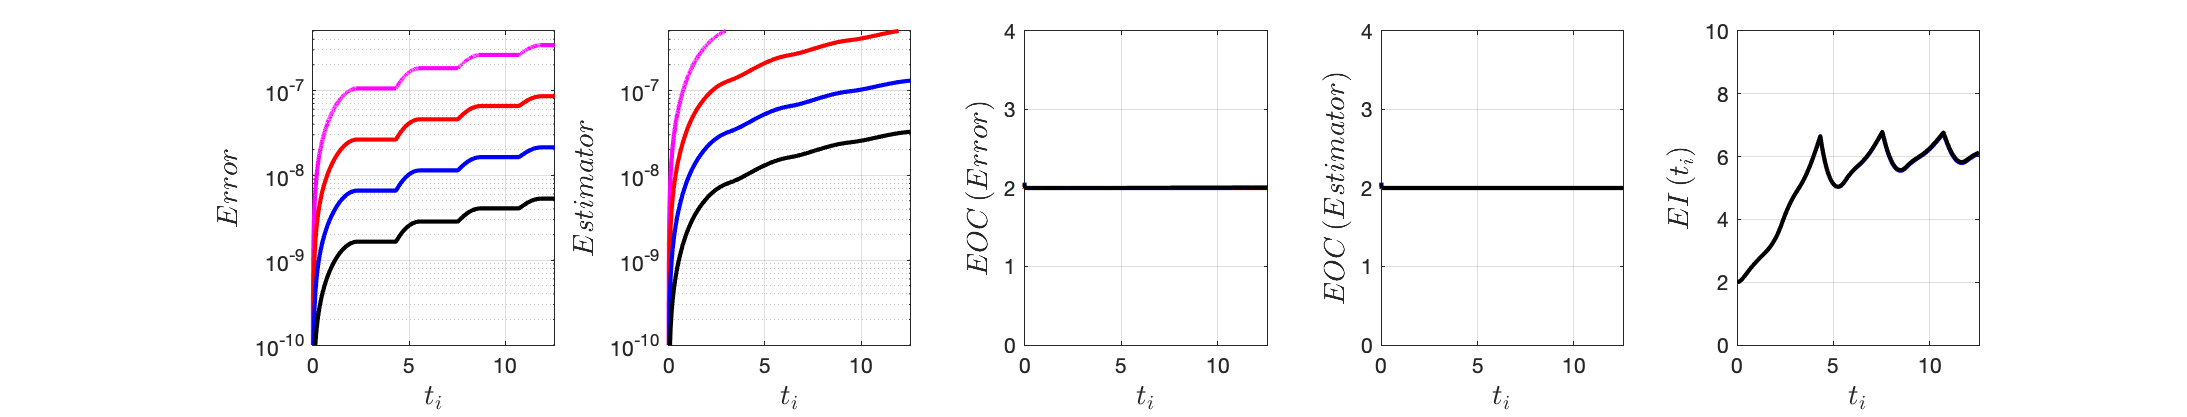
\includegraphics[scale=0.55]{fig_LeapFrogplots_1x5_sin_IC_harmonic_order_2_u10_v0_rec_george}	
	\caption{Reconstruction from Defn. \ref{defn_our_rec}. (from left to right) Error $e_R$ given by (\ref{eq_error_eR}), Estimator $\eta_1$ given by \ref{eq_bound_test}, Error $e_L$ given by  (\ref{eq_error_eL}). EOC error, EOC Estimator, Effectivity Index.}
	\label{fig_all_in_one_our_rec_george_u10_v0}
\end{figure}
\begin{figure}[H]
	\hspace{-3cm}
	%\centering
	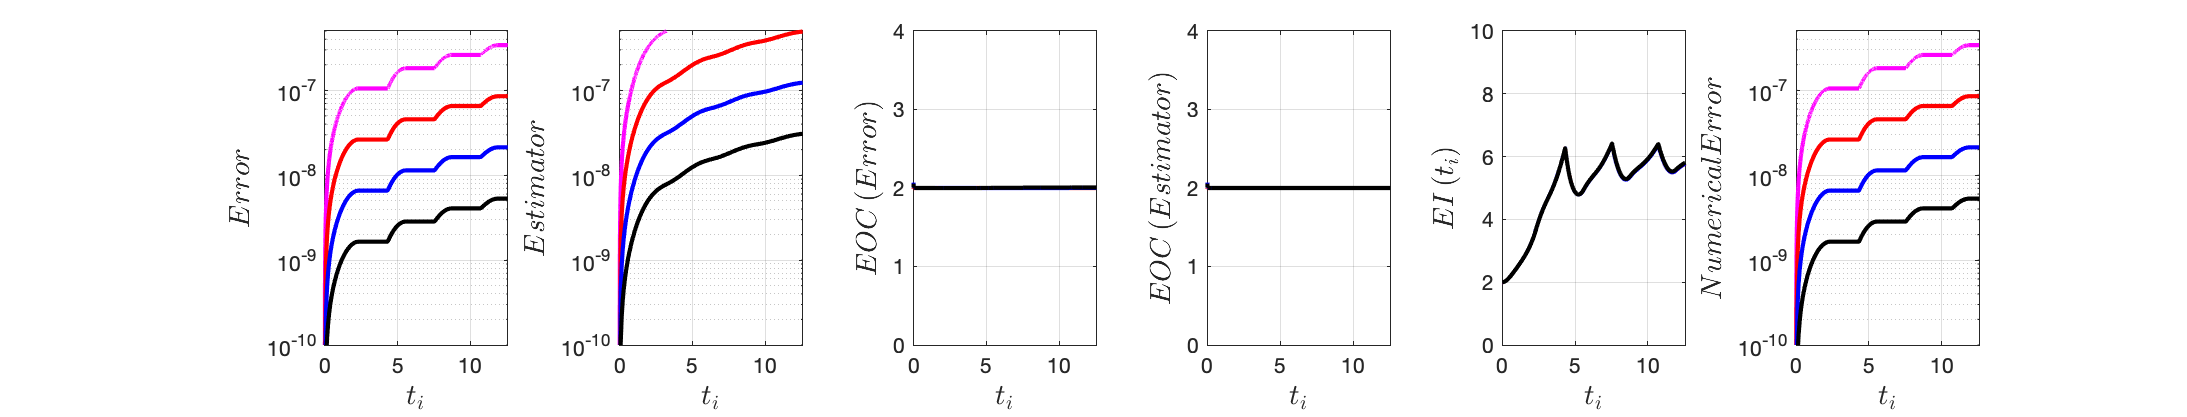
\includegraphics[scale=0.55]{fig_LeapFrogplots_1x5_sin_IC_harmonic_order_2_u10_v0_rec2}	
	\caption{Reconstruction from Defn. \ref{defn_our_rec2}. (from left to right) Error $e_R$ given by (\ref{eq_error_eR}), Estimator $\eta_1$ given by \ref{eq_bound_test}, Error $e_L$ given by  (\ref{eq_error_eL}). EOC error, EOC Estimator, Effectivity Index.}
	\label{fig_all_in_one_our_rec_2_u10_v0}
\end{figure}
\begin{figure}[H]
	\hspace{-3cm}
	%\centering
	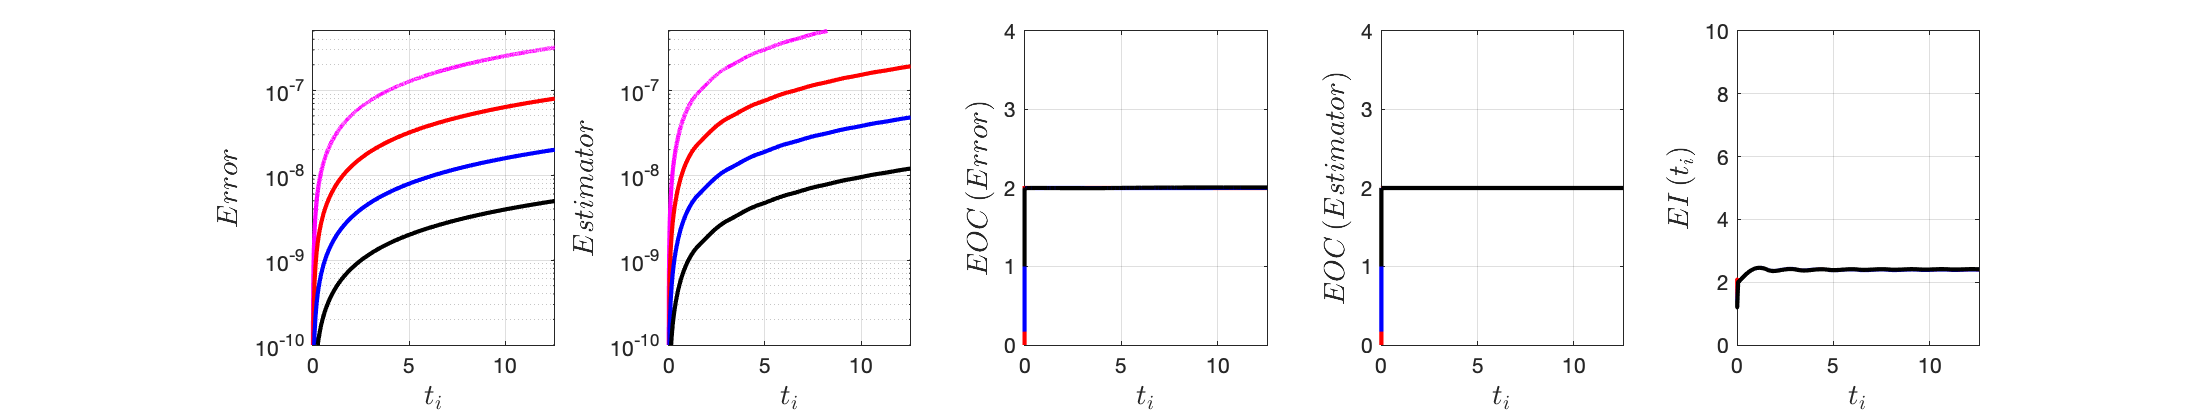
\includegraphics[scale=0.55]{fig_LeapFrogplots_1x5_sin_IC_harmonic_u10_v0_paperrec}	
	\caption{Paper rec. (from left to right) Error $e_R$ given by (\ref{eq_error_eR}), Estimator $\eta_1$ given by \ref{eq_bound_test}, Error $e_L$ given by  (\ref{eq_error_eL}). EOC error, EOC Estimator, Effectivity Index.}
	\label{fig_all_in_one_paperrec_u10_v1}
\end{figure}




\subsection{Discussion}


%%%%%%
In the first set of experiments $\qp{u_0, v_0} = \qp{0,1}$ the reconstruction from \cite{georgoulis2016posteriori} replicates the behaviour of the error more closely than the  reconstructions from Defn. \ref{defn_our_rec} and \ref{defn_our_rec2}.  Between the latter two, the one from Defn. \ref{defn_our_rec2} has a steeper increase.  It is worth noticing that in the reconstruction from Defn.\ref{defn_our_rec}, the initial error does not contribute at all as it is 0.  This manifests in the bound as a calculation of $0/0$ is not allowed and hence, the plot starts from the next pair of values.

In the second set of experiments, $\qp{u_0, v_0} = \qp{1,0}$, the reconstruction from (\ref{defn_our_rec}) performs similarly to that of \cite{georgoulis2016posteriori}.  There appears to be an issue with the reconstruction from Defn. \ref{defn_our_rec2} however, as it is not even a bound from the first 0.5 s.  It is very likely that this is a coding bug.

In the last set of experiments, $\qp{u_0, v_0} = \qp{1,1}$, the reconstruction from (\ref{defn_our_rec2})) outperforms the other two.
\bibliography{apostfd_bibdesk}
\bibliographystyle{ieeetr}
\end{document}